%! Author = idegen
%! Date = 26/11/2021

\documentclass[a4paper]{article}
\usepackage[margin=1in]{geometry}
\usepackage[dvipsnames]{xcolor}
\usepackage[utf8]{inputenc}
\usepackage[english]{babel}
\usepackage[sfdefault]{roboto}
\usepackage[]{amsthm}
\usepackage[]{amssymb}
\usepackage{placeins}
\usepackage{textcomp}
\usepackage{setspace}
\usepackage{fancyhdr}
\usepackage[useregional]{datetime2}
\usepackage{hyperref}
\hypersetup{
    colorlinks=true,
    linkcolor=Emerald,
    filecolor=magenta,
    urlcolor=cyan,
    citecolor=RoyalBlue
}
\usepackage{graphicx}
\usepackage{caption}
\usepackage{subcaption}
\graphicspath{ {./images/} }
\usepackage{textcomp}
\usepackage{outlines}
\usepackage{tabularx}
\usepackage[T1]{fontenc}
\usepackage{scrextend}
\usepackage{multirow}
\makeatletter
\def\namedlabel#1#2{\begingroup
#2%
\def\@currentlabel{#2}%
\phantomsection\label{#1}\endgroup
}
\makeatother

\setlength{\parindent}{0em}
\setlength{\parskip}{0.5em}

\pagestyle{fancy}
\fancyhf{}
\chead{Machine Learning Paradigms}
\rhead{\today}
\lhead{Isabella Degen}
\lfoot{isabella.degen@bristol.ac.uk}
\rfoot{Page \thepage}

\title{Machine Learning Paradigms - Coursework Report}
\author{Isabella Degen - Interactive AI CDT}

\begin{document}
    \maketitle


    \section{Introduction and Approach}\label{sec:introduction}
    My goal for this coursework was to gain more experience with a few ML algorithms, evaluation methods and
    different Python frameworks available. I was also keen to use experiment tracking methods, as
    well as further improve my software engineering practices when writing an ML system. I was less focused on
    finding the best solution for the problem.

    I followed the steps on \href{https://www.kaggle.com/c/morebikes2021/overview/description}{Kaggle}. I wrote a solution
    for both approaches:
    \begin{itemize}
        \item[(a)] separate model for each station
        \item[(b)] single model for all stations together
    \end{itemize}

    The way I setup my scripts made it a simple change of configuration to train a model for all stations or one model
    or either one of them using any ML algorithm.

    I further broke down the work for each of these two approaches into the following steps:
    \subsection*{\label{phs:one}{Phase 1}}
    Predict the availability of bikes for stations 201-275
    \begin{description}
        \item [\namedlabel{itm:phase1-step1}{Step 1.1}] Analyse and investigate the data and decide what ML problem it is
        \item [\namedlabel{itm:phase1-step2}{Step 1.2}] Create an end to end pipeline with a simple model for approach a) and b)
        \item [\namedlabel{itm:phase1-step3}{Step 1.3}] Feature engineering and experiment more with different models
        \item [\namedlabel{itm:phase1-step4}{Step 1.4}] Tune promising setups
    \end{description}

    I submitted models to Kaggle before I did the tuning as I wanted to make sure I got the format right and wanted to
    gain insights on how well my models were performing on the test data.

    \subsection*{\label{phs:two}{Phase 2}}
    Use the pre-trained models for station 1-200 to predict the availability of bikes for stations 201-275
    \begin{description}
        \item [\namedlabel{itm:phase2-step1}{Step 2.1}] Analyse the given models
        \item [\namedlabel{itm:phase2-step2}{Step 2.2}] Create an end to end pipeline for the given models
        \item [\namedlabel{itm:phase2-step3}{Step 2.3}] Investigate the resulting performance and compare to \nameref{phs:one}
    \end{description}

    \subsection*{\label{phs:three}{Phase 3}}
    Combine the approaches from \nameref{phs:one} and \nameref{phs:two}
    \begin{description}
        \item [\namedlabel{itm:phase3-step1}{Step 3.1}] Create an end to end pipeline for the combining the models from \nameref{phs:one} and \nameref{phs:two}
        \item [\namedlabel{itm:phase3-step2}{Step 3.2}] Tune promising setups
        \item [\namedlabel{itm:phase3-step3}{Step 3.3}] Investigate the resulting performance and compare to \nameref{phs:one} and \nameref{phs:two}
    \end{description}

    I keep referring back to these steps in the sections \nameref{sec:technical-background}, \nameref{sec:method}, \nameref{sec:experiment-setup} and
    \nameref{sec:results}. The \nameref{sec:conclusions} sections gives a summary of my overall learnings and conclusions.

    The code for this coursework is available from my GitHub \href{https://github.com/isabelladegen/mlp-2021}{mlp-2021} repository and
    all of the tracked runs are available on my \href{https://wandb.ai/idegen/mlp-2021}{Weights \& Biases - MLP 2021 workspace}.


    \section{Technical Background}\label{sec:technical-background}

    While I wrote my Dialogue and Narrative coursework, I made the painful experience on how quickly a
    simple ML system can get messy. It's
    easy to spend endless time analysing the data in Jupyter Notebooks, running a few experiments, seeing promising results,
    forgetting what the exact setup for those were and then never be able to reproduce them again. Learning from this
    experience I decided to do use hopefully better engineering practices for this coursework. This meant
    that I decided to write all the experiments that went beyond poking around in the data in pure Python. I used test
    driven development to implement the scripts and classes. While the tests are not exhaustive they are touching every
    part of the module and allowed me to find countless mistakes I inevitably made. They also serve as a nice and living
    documentation how to use the different classes and scripts.

    To keep track of the configuration and results for different experiments I used the
    \href{https://wandb.ai/site}{Weights \& Biases platform}\cite{wandb}.
    I shall refer to the Weights \& Biases platform from now on by its Python package name \textit{wandb}. To make full
    use of wandb's capabilities to track experiments I made sure that all hyper parameters,
    conditional processing logic and other magical numbers and strings in the codebase were kept in a configuration
    dataclass that was logged as \texttt{wandb.config}. While initially the purpose for the configuration's dataclass was for experiment
    tracking, it also enabled me to quickly change the setup, run sweeps to tune hyper parameters and other model setups.

    I created a mlp-2021 conda environment on my mac \cite{conda-forge} which can be built and updated using the
    \href{https://github.com/isabelladegen/mlp-2021/blob/main/conda.yml}{conda.yml} file. I only fix the version of Python to 3.9,
    for the other libraries I want to use their newest version. Wandb automatically produces a \texttt{requirements.txt}
    as well as a \texttt{environment.yml} file for each run which lists the exact version of all the libaries an their
    dependencies. This should allow to recreate the exact Python setup used while also making it easy to keep working with
    the newest version unless their should be a reason to fix to a specific version, which I've not come accross for this coursework.

    The \href{https://github.com/isabelladegen/mlp-2021}{Readme} on Github describes how to setup the environment as well
    as how to run the various experiments which can also be seen on on my \href{https://wandb.ai/idegen/mlp-2021}{Wandb - MLP 2021 workspace}.

    Given I was working with simple ML algorithms, I ran all the experiments on my personal laptop.


    \section{Method}\label{sec:method}

    In this section I describe the method used for each of the steps listed in the \nameref{sec:introduction}.

    \subsection*{\nameref{phs:one}}

    For this coursework we were given a dataset for stations 201-275 with 744 labelled samples per station
    resulting in a total 55800 labelled samples. While we were also given a test dataset, the test dataset had no labels
    and therefore could not be used to validate my models during development of the system. For that reason I randomly
    took 10\% of samples away from the 55800 labelled samples. I call the resulting dataset of 5580 labelled data the validation
    dataset and the remaining dataset of 50220 labelled samples the training or dev dataset. All the models are only
    trained on the training dataset. This setup allowed me to verifiy my models performance on unseen data.

    \subsubsection*{\nameref{itm:phase1-step1}}
    The goal for this step is to gain a better idea of what sort of problem we've been given. For this I looked at the
    given dataset on a very high level. I wanted to know how much data we were given, what type of data we were given and
    generally understand
    a bit more what the data means. As I moved to \nameref{itm:phase1-step2} I continued to come back to this step
    to understand more about how many data points were nan to decide how to best pre-process the data for a new column.


    \subsubsection*{\nameref{itm:phase1-step2}}
    As described in \nameref{sec:conclusions} I create a \textit{pipeline} setup where I didn't needed to decide
    on an algorithm and that let me easily experiment and evaluate different models, features and ways of data processing.

    I also wanted to create a baseline. For this I wrote a random estimator that returns a random number of bikes between
    0 and the number of docks for the station.

    Following from that, I created a model for all stations as well as a model per station using the PoissonRegressor from
    scikit-learn \cite{scikit-learn}. The difference between approach a) and b) was a simpler wrapper class that split the
    overall dataframe of all stations back into the data per station and that managed the multiple models. The results
    two can both deal with per station results, overall results and report on per station mean absolut error or
    overall absolute error.

    For both I used bikes\_3h\_ago as feature matrix X. Given 300 rows are missing this value I had to decide what to do
    with a nan value. Possibilities I thought of were: just drop those samples, use the mean number of bikes. I didn't wanted
    to drop 300 samples as I was invevitably going to drop a lot more samples with that strategy when adding more features.
    I decided to put the nan values to the most frequent value. For the per station data that meant to the most frequent for
    the station, for the one model for all stations that meant to the most frequent value overall.

    Given I wanted to make it super easy to swap models and given the results were not great for the PoissonRegressor
    I also added a RandomForestRegressor model from scikit-learn. This made me pull the code out of the PoissonModel class
    into an \texttt{abstract} Model class that is doing the \texttt{fit()} and \texttt{predict()} and creating a result.
    The only bit of code needed for a specific model was the configuration of that model. I reused the same run script
    by passing it the name of the class instead of an instance, so it could create the model itself depending on its configuration.

    For unit testing of the code I used fake data setup in builder classes as well as a smaller data subset of real data.

    I ran a wandb experiment for all of these three naive models: random guessing, poisson regressor and random forest
    regressor with just one feature.

    \subsubsection*{\nameref{itm:phase1-step3}}
    At this point I wanted to include more features into the training to see if I could reduce the prediction error
    especially for the stations that are performing much worse than others. I was still continuing to test both approaches:
    a model per station as well as one model for all stations. However I decided to work with the RandomForestRegressor
    as it was performing better than the PoissonRegressor. I also decided to play with features that I could understand
    what they meant and so I left out the bike profile features (which in hindsight was a mistake).

    Features I wanted to investigate were:
    \begin{itemize}
        \item \textbf{Weather Data}: I'm assuming this is similar across the different stations but could have an impact on
        if people are using more or less motorbikes.
        \item \textbf{Station Data}: For the one model for all station approach it could be beneficial to including station specific data such as longitude
        and latitude, number of docks - bigger stations might be at busier locations than smaller stations, or even just the station id.
        \item \textbf{Situational data}: Weekhour could help help with changes in demand for different times of the day and different days of the week.
        Similarly isHoliday could perhaps help to distinguish between times that have very different demands.
    \end{itemize}

    For each features I needed to decide what pre-processing steps were needed and if and how I could sensibly fill the nan values
    for the feature.

    \subsubsection*{\nameref{itm:phase1-step4}}
    As a final step \nameref{phs:one} I wanted to investigate the impact of hyper parametes on the result. For this I
    ran various used wand's sweep capability. This allowed me to vary the different hyper parameters in congiguration.
    I created a smaller dataset with just 10\% of the data to save runtime as I was interested in the effect of the hyper parameters not
    the final MAE. For the best sweep result I ran a normal experiment on the full dataset. This also lead me to increased
    the sweep dataset to 30\% as the sweep results didn't translate well to the full dataset runs.
    To safe time I only tuned the Random Forest Regressor as it had been consistently outperforming the Poisson Regressor.

    I was most interested in finding a hyper parameter combination that would lessen the overfitting seen in the previous
    experiments. This lead me to try out yet another model from scikit-learn: the MultilayerPerceptronRegressor. Implementing
    it into the code base was simple and followed the same step as describe in \nameref{itm:phase1-step2}.

    \subsection*{\nameref{phs:two}}
    \subsubsection*{\nameref{itm:phase2-step1}}
    To analyse of the given models I inspected the given .csv files. We'd been given simple linear models trained using approach
    a).
    \subsubsection*{\nameref{itm:phase2-step2}}

    Similar to \nameref{itm:phase1-step2} I wrapped the given models in a model class \texttt{BestTrainedModelForAStation}.
    That class implement like the other model classes the \texttt{fit()} and \texttt{predict()} functions and therefore
    could be used in the rest of the pipeline, meaning I could reuse most of the the code from \nameref{itm:phase1-step2} of
    \nameref{phs:one} with a few additions. I modeled the weights in such a way that
    I could calculate the predictions matrix y for each sample by calculating thedot product of each stations feature matrix X
    and the models weight matrix W.

    For the pretrained models from station 1-200, I used the training dataset for models 2001-275 to calculate the MAE for
    each of the pretrained models would achieve for each station 201-275. I'd then select the the pretrained model with
    the lowest MAE to be used as estimator for each of the stations 201-275. I could reuse the same \texttt{StationPerModel}
    class from \nameref{phs:one} to keep track of which model to use for each station.

    \subsubsection*{\nameref{itm:phase2-step3}}

    To investigate how well this approach of using the pretrained models to predict the number of bikes for stations 201-275
    did I used the validation dataset to do predictions for data that had not been used to select the pretrained model.
    I calculated the MAE the same way as I'd been doing and the run was logged on wand db like it had been
    for other models from \nameref{phs:one}.

    \subsection*{\nameref{phs:three}}
    \subsubsection*{\nameref{itm:phase3-step1}}
    In this step I combined the best model from \nameref{phs:one} with the best pretrained model as created in \nameref{phs:two}
    by letting both models make an estimation and using the average of the two estimates as prediction of bikes for the combined model.
    For this I created a new run script that would train both models, then predict using the validation and then
    combine the results. I extended the existing \texttt{PredictionResult} class to be able to do such a combination.

    \subsubsection*{\nameref{itm:phase3-step2}}
    I ran a few more sweeps, mainly to tune the Multilayer Perceptron Model. Seeing that the pretrained
    models were using the bikes profile features I also stared to use those features in my multilayer perceptron model as
    they did perform better than the other features.

    \subsubsection*{\nameref{itm:phase3-step3}}
    I used the same method as I've used for \nameref{phs:one} and \nameref{phs:two} to investigate and compare the
    overal results.

%%%%%%%%%%%%%%%%%%%%%%%%%%%%%%%%%%%%%%%%%%%%%%


    \section{Experiment Setup}\label{sec:experiment-setup}
    I'm using the JetBrains DataSpell IDE for working with Notebooks and PyCharm IDE for working with Python. Both IDEs offer
    a rich debugging and runtime environment, test and script execution and advanced refactoring abilities.

    \subsection*{\nameref{phs:one}}

    \subsubsection*{\nameref{itm:phase1-step1}}
    I mostly used the
    \href{https://github.com/isabelladegen/mlp-2021/blob/main/notebooks/ExperimentWithPerStationData.ipynb}{ExperimentWithPerStationData.ipynb}
    Jupyter notebook and loaded the data into a pandas dataframe \cite{reback2020pandas} which overs various methods
    to get a quick insights of the data such as: \texttt{info()}, \texttt{describe()} and \texttt{value\_counts()} as well
    as methods to count nan's.

    \subsubsection*{\nameref{itm:phase1-step2}}
    All the code for the pipeline is just pure Python and can be found in the
    \href{https://github.com/isabelladegen/mlp-2021/tree/main/src}{src} folder on GitHub. There are two
    scripts to run either the random estimator or a model based estimator:
    \begin{enumerate}
        \item \href{https://github.com/isabelladegen/mlp-2021/blob/main/src/random_predictions.py}{random\_predictions.py}:
        It uses the \href{https://github.com/isabelladegen/mlp-2021/blob/c48d85dc364b5a2e7e59f16961b32f9e6c245735/src/models/RandomEstimator.py}{RandomEstimator}
        class to estimate a random number of bikes
        \item \href{https://github.com/isabelladegen/mlp-2021/blob/main/src/simple_regression.py}{simple\_regression.py}: It creates
        an instance of the \href{https://github.com/isabelladegen/mlp-2021/blob/main/src/models/Model.py}{Model} class given, which
        can be either for this experiment was either the \href{https://github.com/isabelladegen/mlp-2021/blob/main/src/models/PoissonModel.py}{PoissonModel}
        or the \href{https://github.com/isabelladegen/mlp-2021/blob/main/src/models/RandomForestRegressorModel.py}{RandomForestRegressorModel}.
    \end{enumerate}

    Each model implements \texttt{predict()} which returns a  \href{https://github.com/isabelladegen/mlp-2021/blob/c48d85dc364b5a2e7e59f16961b32f9e6c245735/src/PredictionResult.py}{PredictionResult}
    class that is used for evaluation of the model. It calculates the overall mean absolute error (MAE) using \texttt{mean\_absolute\_error}
    from scikit-learn, as well as the the MAE for each station. Furthermore the result also implements the
    \texttt{write\_to\_csv()} function that writes the predictions to a csv file using the format required for the Kaggle submissions.

    The \texttt{run} script calls \texttt{wandb.init(...)} to start the experiment tracking, loads the training data using the required data,
    creates both a single model and a model per station depending on the configuration, trains the model calling \texttt{fit()},
    predicts the number of bikes for the training, validation and test data sets calling the different models \texttt{predict(...)}
    functions which each return a prediction result, which is then called to log the overall MAE as well as the per
    station MAE for the training and validation dataset, this is logged to wanddb using \texttt{wandb.log(...)} and finally
    the script creates a csv for a Kaggle submission. All the rest of the experiment is automatically tracked by wandb
    and the results can be visualised on there.

    The \href{https://github.com/isabelladegen/mlp-2021/blob/c48d85dc364b5a2e7e59f16961b32f9e6c245735/src/Data.py}{Data} class
    is used to load all the data and also does all of the pre-processing based on configuration values. It encapsulates
    a pandas dataframe and provides easy access function to get the feature matrix X and the labelled data y. It's further
    capable of operating on all data or of returning a Data class for each station. The Data class is loading the
    bikes\_3h\_ago column as pandas \texttt{category} type and is using the
    \texttt{SimpleImputer(strategy="most\_frequent")} from scikit-learn to fill the nan values for bikes\_3h\_ago.

    Finally all the configurations are stored in the Configurations dataclass defined in
    \href{https://github.com/isabelladegen/mlp-2021/blob/c48d85dc364b5a2e7e59f16961b32f9e6c245735/src/configurations.py}{configurations.py}.
    This script also provides a TestConfiguration class that disables the upload to wandb for unit testing purposes but
    still ensures the calls are syntactically correct. At this stage both the PoissonRegressor as well as the RandomForestRegressor
    were using their default configurations. However,
    I've already made these hyper parameters configurable so that they automatically get logged in wandb.

    Finally, I wrote a helper \href{https://github.com/isabelladegen/mlp-2021/blob/c48d85dc364b5a2e7e59f16961b32f9e6c245735/src/create_dev_and_validation_csv.py}{script}
    to create the training and validation dataset and write them as .csv files in my local
    data folder. Each experiment is using the same training and validation datasets, loading them from these .csv files.

    The code as evolved since this experiment, the hashes listed below can be used to get the versions at the time of
    these first simple experiment runs:

    \begin{itemize}
        \item \textbf{Random Prediction}: \\git checkout -b "classic-sun-10"\footnote{\label{fn:wand-db-name}wandb run name} c22db5e7b461cfd7ba7e7af81460d93b984b2e14
        \item \textbf{Poisson Regressor}: \\git checkout -b "chocolate-serenity-19"\footref{fn:wand-db-name} e1c7158a2f41568b7781d00cc0d5330982edc398
        \item \textbf{Random Forest Regressor}: \\git checkout -b "peach-bird-23"\footref{fn:wand-db-name} e6e86614d7e62a3f09bd635c8125f479c0d4e971
    \end{itemize}

    \subsubsection*{\nameref{itm:phase1-step3}}
    The underlying infrastructure was in place by from the previous step. All I needed to do is change the configurations
    and decide what to do with the nan values. I used the
    \href{https://github.com/isabelladegen/mlp-2021/blob/c48d85dc364b5a2e7e59f16961b32f9e6c245735/notebooks/TestAndTrainingDataForFeatureSelection.ipynb}{TestAndTrainingDataForFeatureSelection.ipynb}
    Jupyter notebook to find get some high level statistics about the features I was about to add. I decided early
    on (and mistakenly) not to include the bike profile features due to the many nan values. The location feature investigation is
    in the \href{https://github.com/isabelladegen/mlp-2021/blob/c48d85dc364b5a2e7e59f16961b32f9e6c245735/notebooks/InvestigateFeatures.ipynb}{InvestigateFeatures.ipynb}
    Jupyter notebook.

    I mostly used the RandomForestRegressor for this investigation. Table \ref{tbl:feature-exploration-overview} gives an
    overview of the different
    features explored as well as a link to the wandb logs for each of the relevant run. While analysing the
    weather data I noticed that precipitation had no training data at all and was therefore not going to be useful for training and
    the ranges of temperature between the training and the test dataset did not overlap well so I decided to leave that out
    for now too.

    \begin{table}[h]
        \centering
        \begin{tabularx}{\textwidth}{|X|X|X|X|}
            \hline
            \textbf{Feature (s)}                                                    & \textbf{\#nan}                                                  & \textbf{Type} & \textbf{Experiment Id}                                                                         \\ \hline
            numDocks                                                                & no nan                                                          & category      & \href{https://wandb.ai/idegen/mlp-2021/runs/185f8iiz?workspace=user-idegen}{autumn-rain-25}    \\ \hline
            station                                                                 & no nan                                                          & category      & \href{https://wandb.ai/idegen/mlp-2021/runs/3ikbmzvm?workspace=user-idegen}{wobbly-hill-29}    \\ \hline
            weekhour                                                                & no nan                                                          & category      & \href{https://wandb.ai/idegen/mlp-2021/runs/36vs3wjd?workspace=user-idegen}{easy-capybara-30}  \\ \hline
            windMeanSpeed.m.s, windDirection.grades, relHumidity.HR, airPressure.mb & all each had the same 75 samples with nan, fill with mean value & float         & \href{https://wandb.ai/idegen/mlp-2021/runs/2ncnkrj2?workspace=user-idegen}{vital-hill-32}     \\ \hline
            isHoliday                                                               & 75 nan, fill with most frequent value                           & category      & \href{https://wandb.ai/idegen/mlp-2021/runs/140v0dji?workspace=user-idegen}{astral-feather-33} \\ \hline
        \end{tabularx}
        \caption{Overview of features explored, strategy for how to fill nan and link to the experiment on wanddb.}
        \label{tbl:feature-exploration-overview}
    \end{table}


    \subsubsection*{\nameref{itm:phase1-step4}}

    To be able to run sweeps I crated the \href{https://github.com/isabelladegen/mlp-2021/blob/fba40c1f27f066e1c5413c45a50c90a32a018f81/src/sweep.py}{sweep.py}
    script which sets up all the parameters to sweep, any parameter not overwritten by the
    sweep configuration will be used from the standard configuration. When sweeping I'm not doing running the test
    predictions.

    Varying too many parameters at once can quickly become overwhelming. Therefore I only varied a few values per sweep
    and iterated with what seemed to be working best. The results sections has links to all the sweep results which also contain the setup.


    \subsection*{\nameref{phs:two}}
    To be able to reuse as much of the code from \nameref{phs:one} I created a
    \href{https://github.com/isabelladegen/mlp-2021/blob/fba40c1f27f066e1c5413c45a50c90a32a018f81/src/models/BestPreTrainedModelForAStation.py}{BestPreTrainedModelForAStation.py}
    class that had the same method as the other models but with custom \texttt{fit()} and \texttt{predict()} methods.
    This class is remembering which of the models from the \href{https://github.com/isabelladegen/mlp-2021/blob/fba40c1f27f066e1c5413c45a50c90a32a018f81/src/Data.py#L29}{PretrainedLinearModel}
    class produces the lowest MAE for the training data. It then uses this pretrained model to predict the numbers of bikes.
    The \texttt{PretrainedLinearModel} loads all the model's csv files into pandas dataframe. The same but extended
    \href{https://github.com/isabelladegen/mlp-2021/blob/fba40c1f27f066e1c5413c45a50c90a32a018f81/src/models/PerStationModel.py}{PerStationModel.py}
    class is used manage the per station model setup. \href{https://github.com/isabelladegen/mlp-2021/blob/fba40c1f27f066e1c5413c45a50c90a32a018f81/src/predict_using_trained_models.py}{predict\_using\_trained\_models.py}
    is the new run script. It uses the same \texttt{train\_predict\_evaluate\_log\_for\_model\_and\_data()} function
    as the other run script but has a slightly different setup to create the \texttt{PretrainedLinearModel} class.


    \subsection*{\nameref{phs:three}}

    To be able to combine MAE from too models the existing I extend the \href{https://github.com/isabelladegen/mlp-2021/blob/fba40c1f27f066e1c5413c45a50c90a32a018f81/src/PredictionResult.py}{PredictionResult}
    class. I also wrote a new run script \href{https://github.com/isabelladegen/mlp-2021/blob/fba40c1f27f066e1c5413c45a50c90a32a018f81/src/predict_using_pretrained_and_my_own_model.py}{predict\_using\_pretrained\_and\_my\_own\_model.py}
    that rains both the pre trained model (to find the one best matching the station) and the multilayer perceptron regressor model
    and logs the results to wandb. Other than that the code could be reused from \nameref{phs:one}.


%%%%%%%%%%%%%%%%%%%%%%%%%%%%%%%%%%%%%%%%%%%


    \section{Results}\label{sec:results}
    \subsection*{\nameref{phs:one}}
    \subsubsection*{\nameref{itm:phase1-step1}}
    The dataset we are given has 55875 samples. 75, exactly one per station, of these samples are missing their label ('bikes'
    column value null).
    I decided to simply exclude those rows, meaning I had in total 55800 labelled samples, 744 per station. Furthermore,
    13275 rows have a least one nan value in other columns.
    We've been given various information:
    \begin{itemize}
        \item \textbf{Information about the station}: tation (station id), latitude, longitude and
        numDocks (number of available bike docks)
        \item \textbf{Information about the time when the sample was taken}: timestamp, year, month, day, hour,
        weekday, weekhour (a combination of weekday and hour), isHoliday (marking public holidays)
        \item \textbf{Information about the weather}: windMaxSpeed.m.s, windMeanSpeed.m.s,  windDirection.grades,
        temperature.C, relHumidity.HR, airPressure.mb, precipitation.l.m2
        \item \textbf{Information about the bike usage}: bikes\_3h\_ago, full\_profile\_3h\_diff\_bikes,
        full\_profile\_bikes, short\_profile\_3h\_diff\_bikes, short\_profile\_bikes, bikes
    \end{itemize}

    Other than the information about the bike usage, these all made sense. I'm to this day not sure what the columns
    about the bike usage actually mean other than bikes\_3h\_ago persumably is the number of bikes at the station 3h
    before the sample was taken and bikes is the number of bikes at the station when the sample was taken. Curiously it
    is possible for a station to have and record more bikes than the number of docks available.

    Not all data types are useful in their raw format. E.g weekday would need to be translated into a numerical value.
    Other than the weather data the given data was categorical.

    \subsubsection*{\nameref{itm:phase1-step2}}

    I ran multiple experiments for Random Guessing, basic Poisson Regressor and Random Forest Regressor, however
    representative runs on wandb are listed below as reference for the results and configurations used, further runs can
    be found e.g using tags:
    \begin{itemize}
        \item \href{https://wandb.ai/idegen/mlp-2021/runs/3k64fgcw/overview?workspace=user-idegen}{Random Guessing} - classic-sun-10
        \item \href{https://wandb.ai/idegen/mlp-2021/runs/1iyx8zmh/overview?workspace=user-idegen}{Poisson Regressor} - chocolate-serenity-19
        \item \href{https://wandb.ai/idegen/mlp-2021/runs/25zvoihx/overview?workspace=user-idegen}{Random Forest Regressor} -peach-bird-23
    \end{itemize}

    Table \ref{tbl:phase1-step2-simple-model-mae} shows that random guessing is in average 7 bikes off, while both ML models
    outperformed random guessing and were only around 3 bikes off. The random forest regressor performed slightly better and
    for both ML models the model per station peformed better than a single model for all stations. All models
    were reasonable quick to train and run: random guessing took 8s, 1m 55s and the Random Forest Regressor took 11m 7s.
    These timings are to be taken with a pinch of salt as the experiment was run on my machine with many other applications
    running at the same time. They can only be used to get a general feeling. If of interest, wandb does
    also log CPU, memory and disk utilisation. For the two ML models the time includes both training of the single model
    as well as training of a model per station.

    \begin{table}[h]
        \centering
        \begin{tabularx}{\textwidth}{|X|XX|XX|XX|}
            \hline
            \multirow{2}{*}{MAE} & \multicolumn{1}{l|}{Random Guessing} & & \multicolumn{2}{l|}{Poisson Regressor} & \multicolumn{2}{l|}{Random Forest Regressor} \\ \cline{2-7}
            & \multicolumn{1}{l|}{Training} & Validation & \multicolumn{1}{l|}{Training} & Validation & \multicolumn{1}{l|}{Training} & Validation \\ \hline
            a) Model per station & \multicolumn{2}{l|}{\multirow{2}{*}{7.369}} & \multicolumn{1}{l|}{3.236}    & 3.327      & \multicolumn{1}{l|}{2.907}    & 3.146      \\ \cline{1-1} \cline{4-7}
            b) One Model & \multicolumn{2}{l|}{} & \multicolumn{1}{l|}{3.767} & 3.812 & \multicolumn{1}{l|}{3.198}    & 3.281      \\ \hline
        \end{tabularx}
        \caption{MAE for Random Guessing, Poisson Regressor and Random Forest Regressor. Last two using default configuration and one feature bikes\_3h\_ago. For
        Random Guessing the dataset was used as one Training \& Validation as nothing is learned from the data.}
        \label{tbl:phase1-step2-simple-model-mae}
    \end{table}

    Figure \ref{fig:simple-pr-rfr-mae-perstation} shows the MAE results for both the Poisson Regressor as well as the
    Random Forest Regressor. Both models do better on the training data then the validation data and both models do
    better for a model per station compared to one model. Station 233 performs the worst and has an MAE of 10 for the
    Poisson Regressor and 7.9 for the Random Forest Regressor for a per station model. The error is even bigger with the
    one model approach for both algorithms. And there are stations that are doing better than average: 209-211, 213, 227,
    252, 256-259, 262, 265-270, 272-275 and have an MAE around 2 for the Random Forest Regressor.

    The stations that perform consistently the worst are:
    \begin{itemize}
        \item Station 233: PoissonRegressor run classic-pyramid-22 - MAE 11.6
        \item Station 249: PoissonRegressor run classic-pyramid-22 - MAE 11.25
        \item Station 208: PoissonRegressor run classic-pyramid-22 - MAE 7.7
        \item Station 230: PoissonRegressor run classic-pyramid-22 - MAE 7.6
    \end{itemize}

    \begin{figure}[h]
        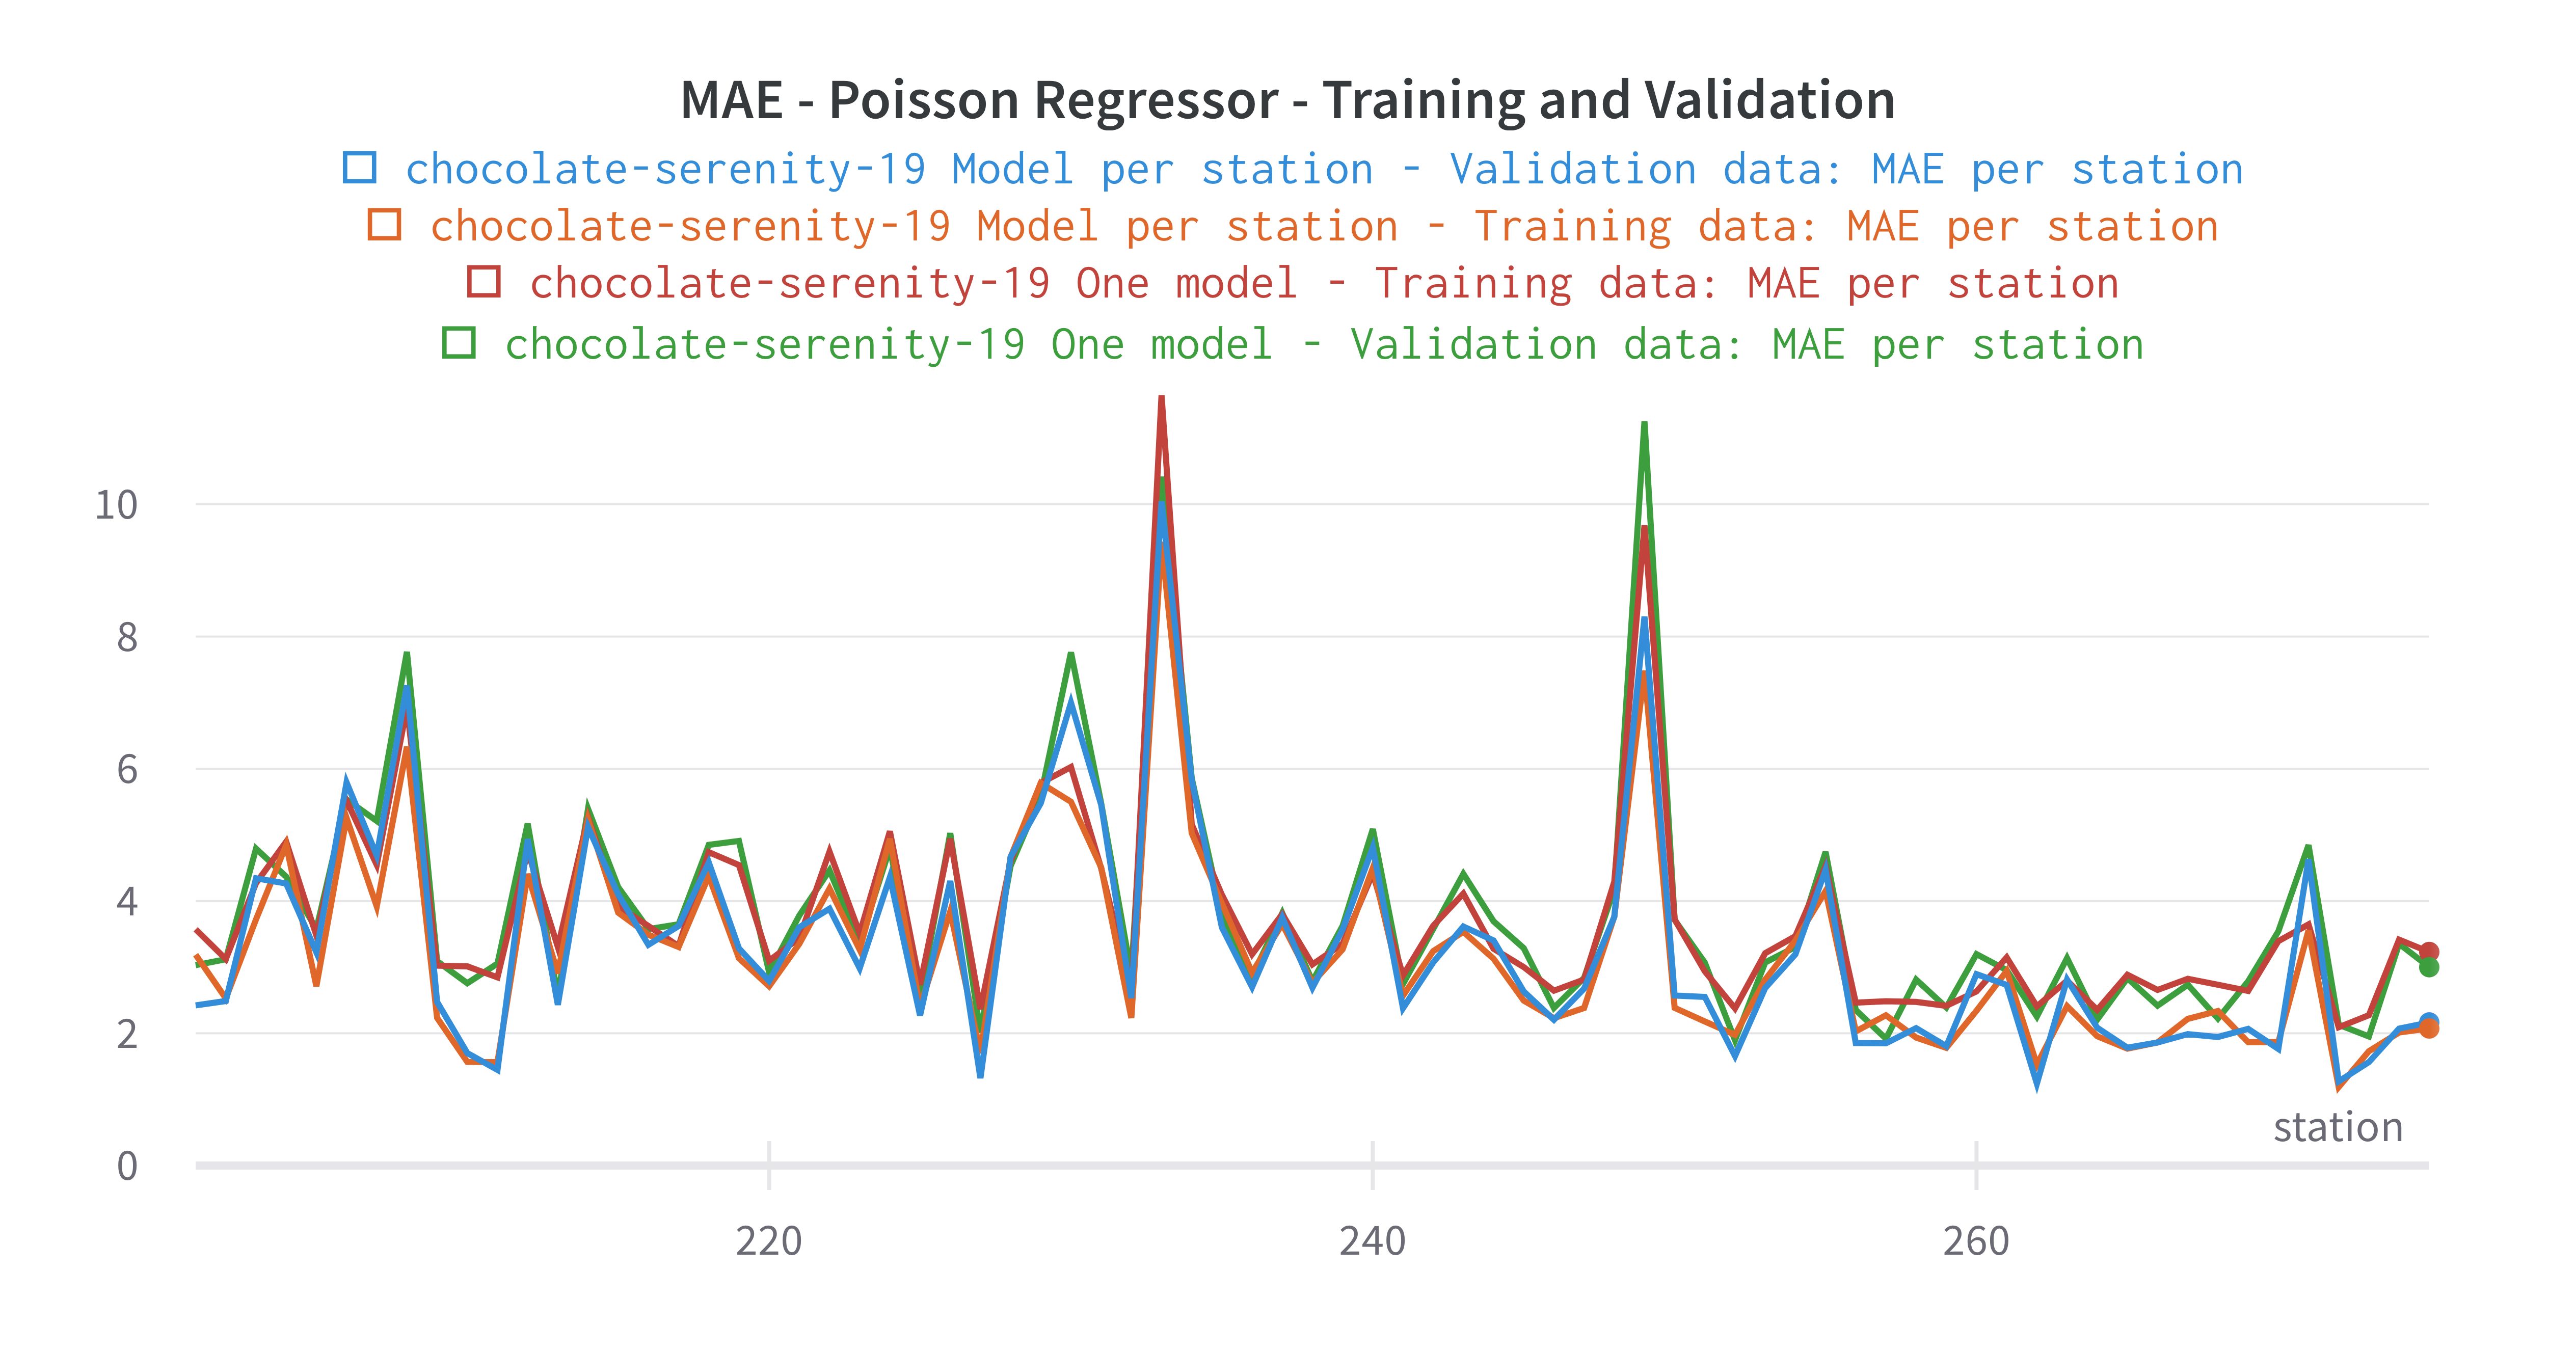
\includegraphics[width=0.5\textwidth]{mae-pr-perstation}\hfill
        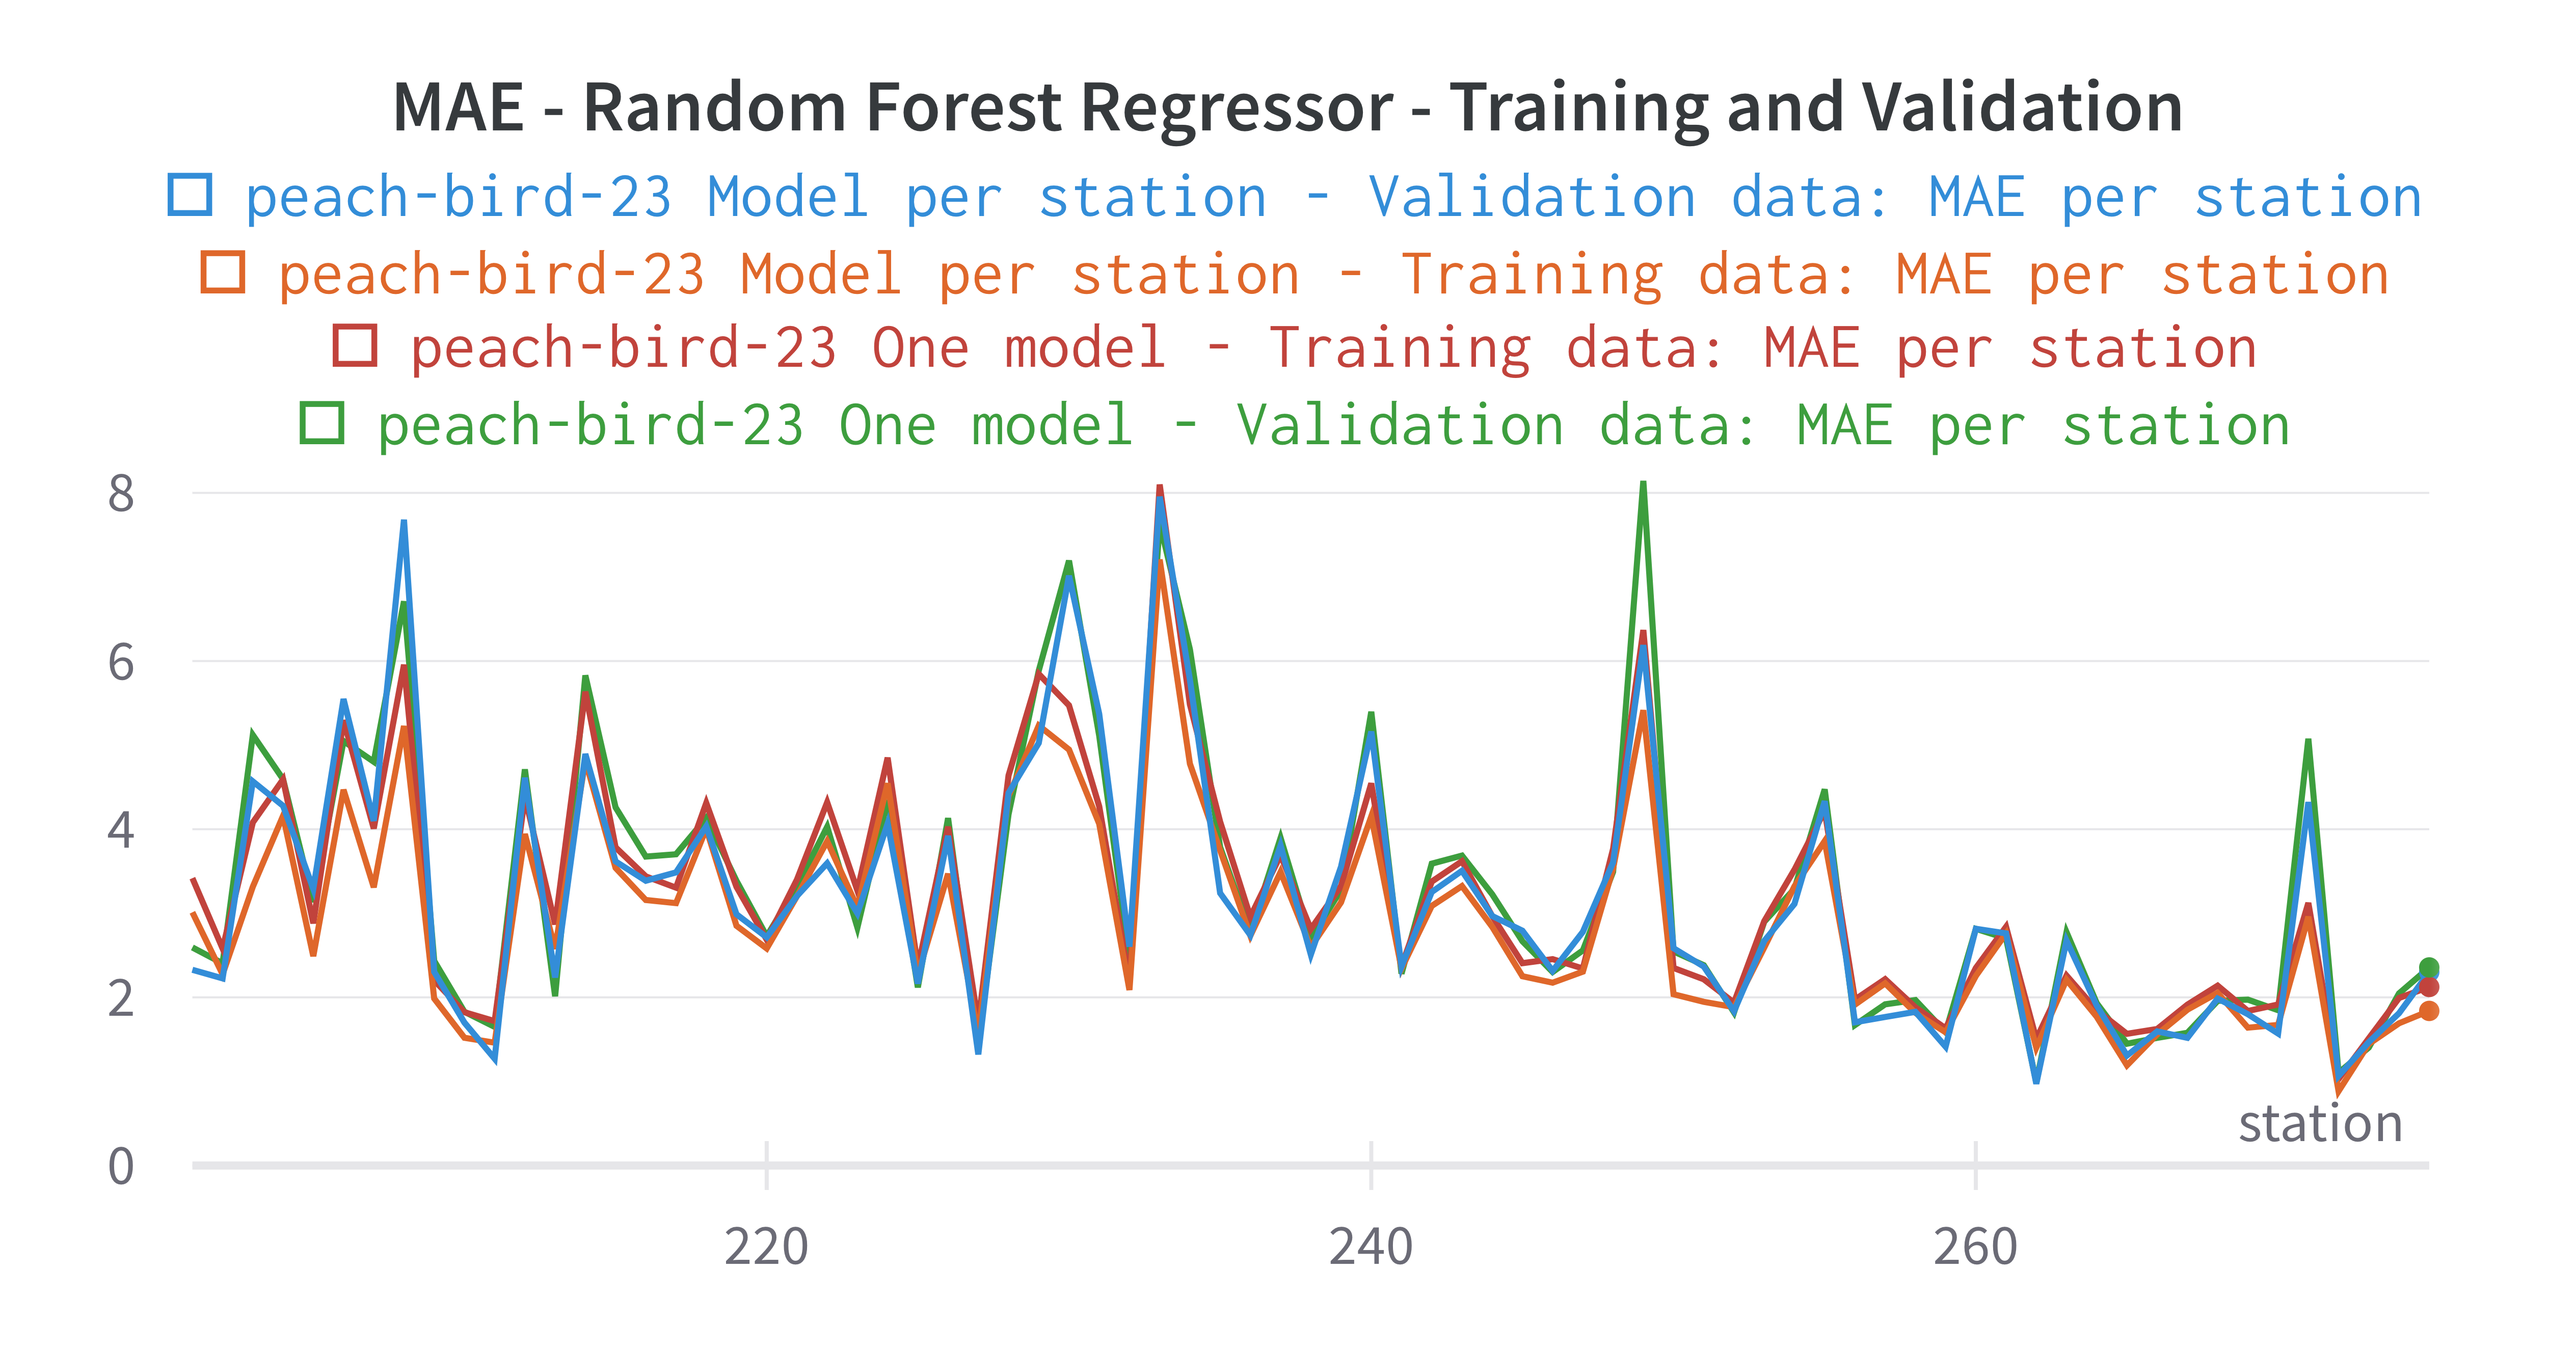
\includegraphics[width=0.5\textwidth]{mae-rfr-comparison}
        \caption{MAE per station for training and validation dataset for both model per station and a single model}
        \label{fig:simple-pr-rfr-mae-perstation}
    \end{figure}


    \subsubsection*{\nameref{itm:phase1-step3}}

    Table \ref{tbl:phase1-step3-runs-mae} shows the MAEs for the RandomForestRegressor with different features, for more
    details follow the link to the experiment on wandb.

    Effects of the different features were as following:
    \begin{itemize}
        \item  Adding the number of docks as expected made a difference for
        the one model for all stations but made the model per station perform less well.
        \item Adding the station made the one model for all stations perform even better but did as expected not improve
        the model per station. The effect was better for the training dataset but not necessarily for the validation.
        \item Adding the weekhour had a big impact on both approaches for the training dataset almost halved the MAE.
        The impact on the validation dataset was also significant but not quite as pronounced and this is the start of the
        increase in different MAEs for the training dataset and validation dataset
        \item Adding the different weather features improved the MAE for the training dataset but worsened it for the validation
        dataset. The model seems to start to overfit to the training data.
        \item Removing the weather data but adding isHoliday was a further improvement on adding weekhour but only for the Model
        per station. For the one model, while doing better on the training dataset it performed worse on the validation dataset
        than only using weekhour.
    \end{itemize}

    \begin{table}[h]
        \begin{tabularx}{\textwidth}{|X|p{0.3\textwidth}|XXX|XX|}
            \hline
            \multirow{2}{*}{Run} &
            \multirow{2}{*}{Features} &
            \multicolumn{3}{l|}{a) Model per station} &
            \multicolumn{2}{l|}{b) One Model} \\ \cline{3-7}
            &
            &
            \multicolumn{1}{l|}{Training} &
            \multicolumn{1}{l|}{Validation} &
            Test &
            \multicolumn{1}{l|}{Training} &
            Validation \\ \hline
            \href{https://wandb.ai/idegen/mlp-2021/runs/185f8iiz?workspace=user-idegen}{autumn-rain-25} &
            bikes\_3h\_ago, numDocks &
            \multicolumn{1}{l|}{2.907} &
            \multicolumn{1}{l|}{3.147} &
            - &
            \multicolumn{1}{l|}{3.124} &
            3.269 \\ \hline
            \href{https://wandb.ai/idegen/mlp-2021/runs/3ikbmzvm?workspace=user-idegen}{wobbly-hill-29} &
            station, bikes\_3h\_ago, numDocks &
            \multicolumn{1}{l|}{2.907} &
            \multicolumn{1}{l|}{3.146} &
            - &
            \multicolumn{1}{l|}{2.918} &
            3.149 \\ \hline
            \href{https://wandb.ai/idegen/mlp-2021/runs/36vs3wjd?workspace=user-idegen}{easy-capybara-30} &
            station, bikes\_3h\_ago, numDocks, weekhour &
            \multicolumn{1}{l|}{1.052} &
            \multicolumn{1}{l|}{2.262} &
            2.923 &
            \multicolumn{1}{l|}{1.181} &
            2.53 \\ \hline
            \href{https://wandb.ai/idegen/mlp-2021/runs/2ncnkrj2?workspace=user-idegen}{vital-hill-32} &
            station, bikes\_3h\_ago, numDocks, weekhour, windMeanSpeed.m.s, windDirection.grades, relHumidity.HR, airPressure.mb &
            \multicolumn{1}{l|}{0.9105} &
            \multicolumn{1}{l|}{2.512} &
            - &
            \multicolumn{1}{l|}{1.109} &
            2.875 \\ \hline
            \href{https://wandb.ai/idegen/mlp-2021/runs/140v0dji?workspace=user-idegen}{astral-feather-33} &
            station, bikes\_3h\_ago, numDocks, weekhour, isHoliday &
            \multicolumn{1}{l|}{1} &
            \multicolumn{1}{l|}{2.219} &
            2.885 &
            \multicolumn{1}{l|}{1.137} &
            2.482 \\ \hline
        \end{tabularx}
        \caption{MAE for the Random Forest Regressor with different features}
        \label{tbl:phase1-step3-runs-mae}
    \end{table}

    \begin{figure}[h]
        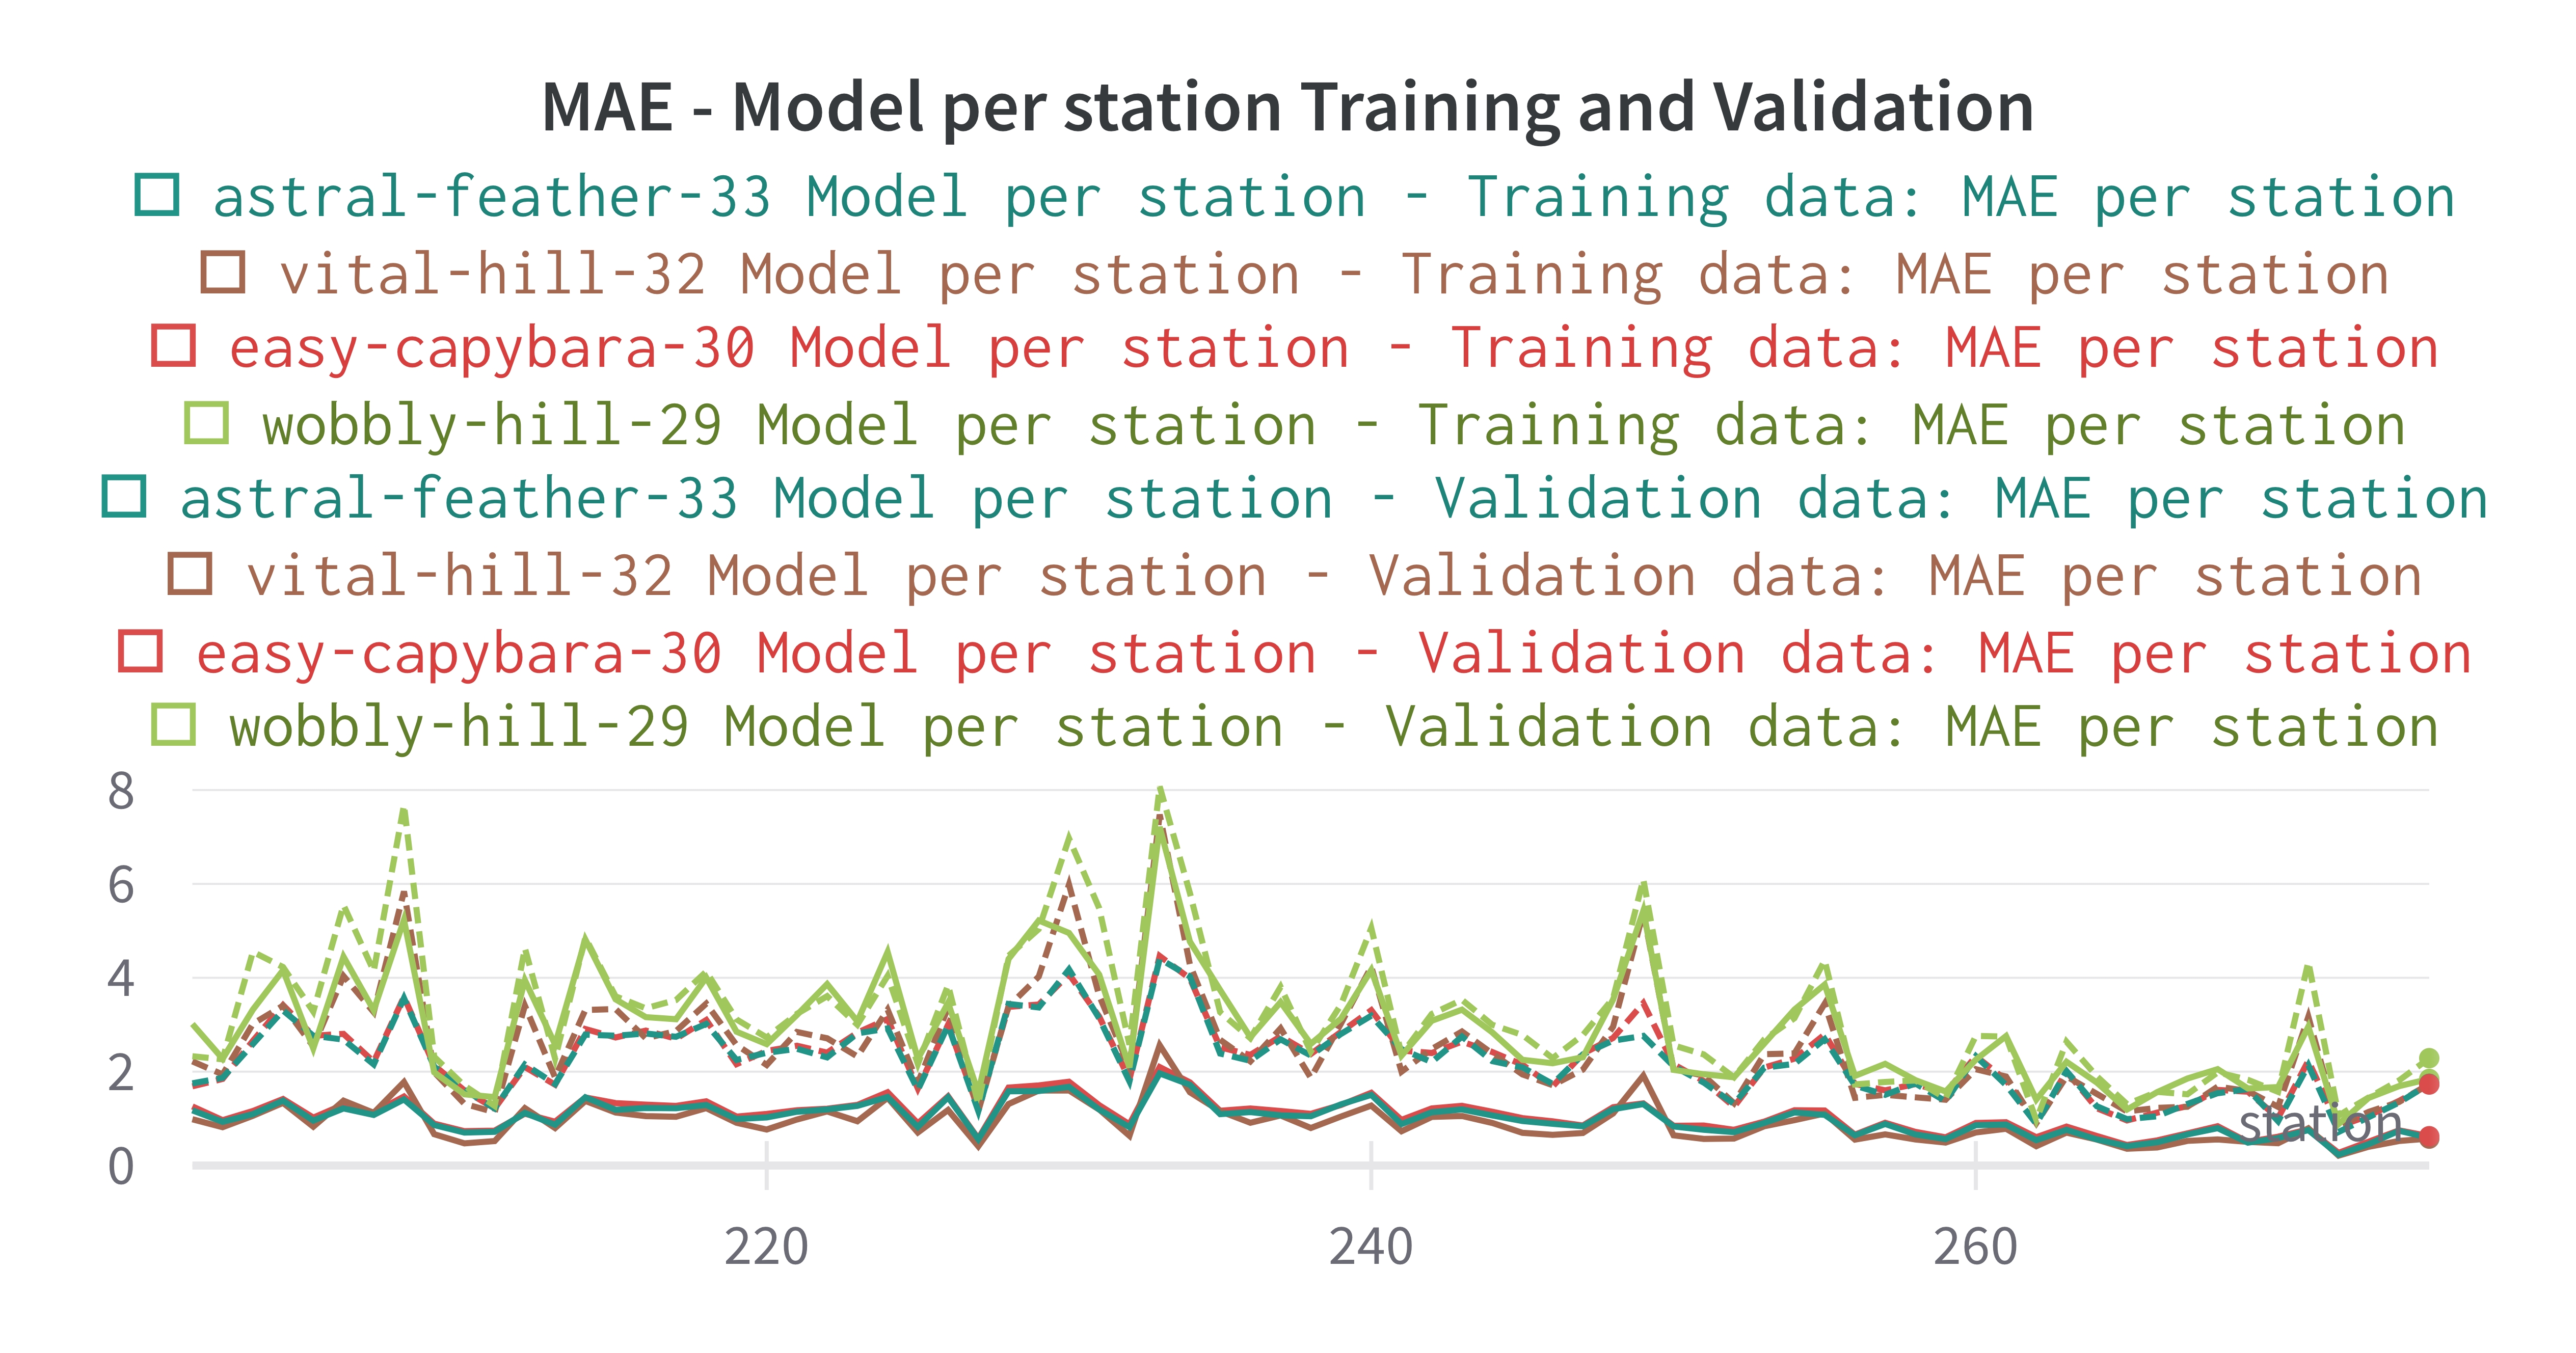
\includegraphics[width=0.5\textwidth]{mae-step3}\hfill
        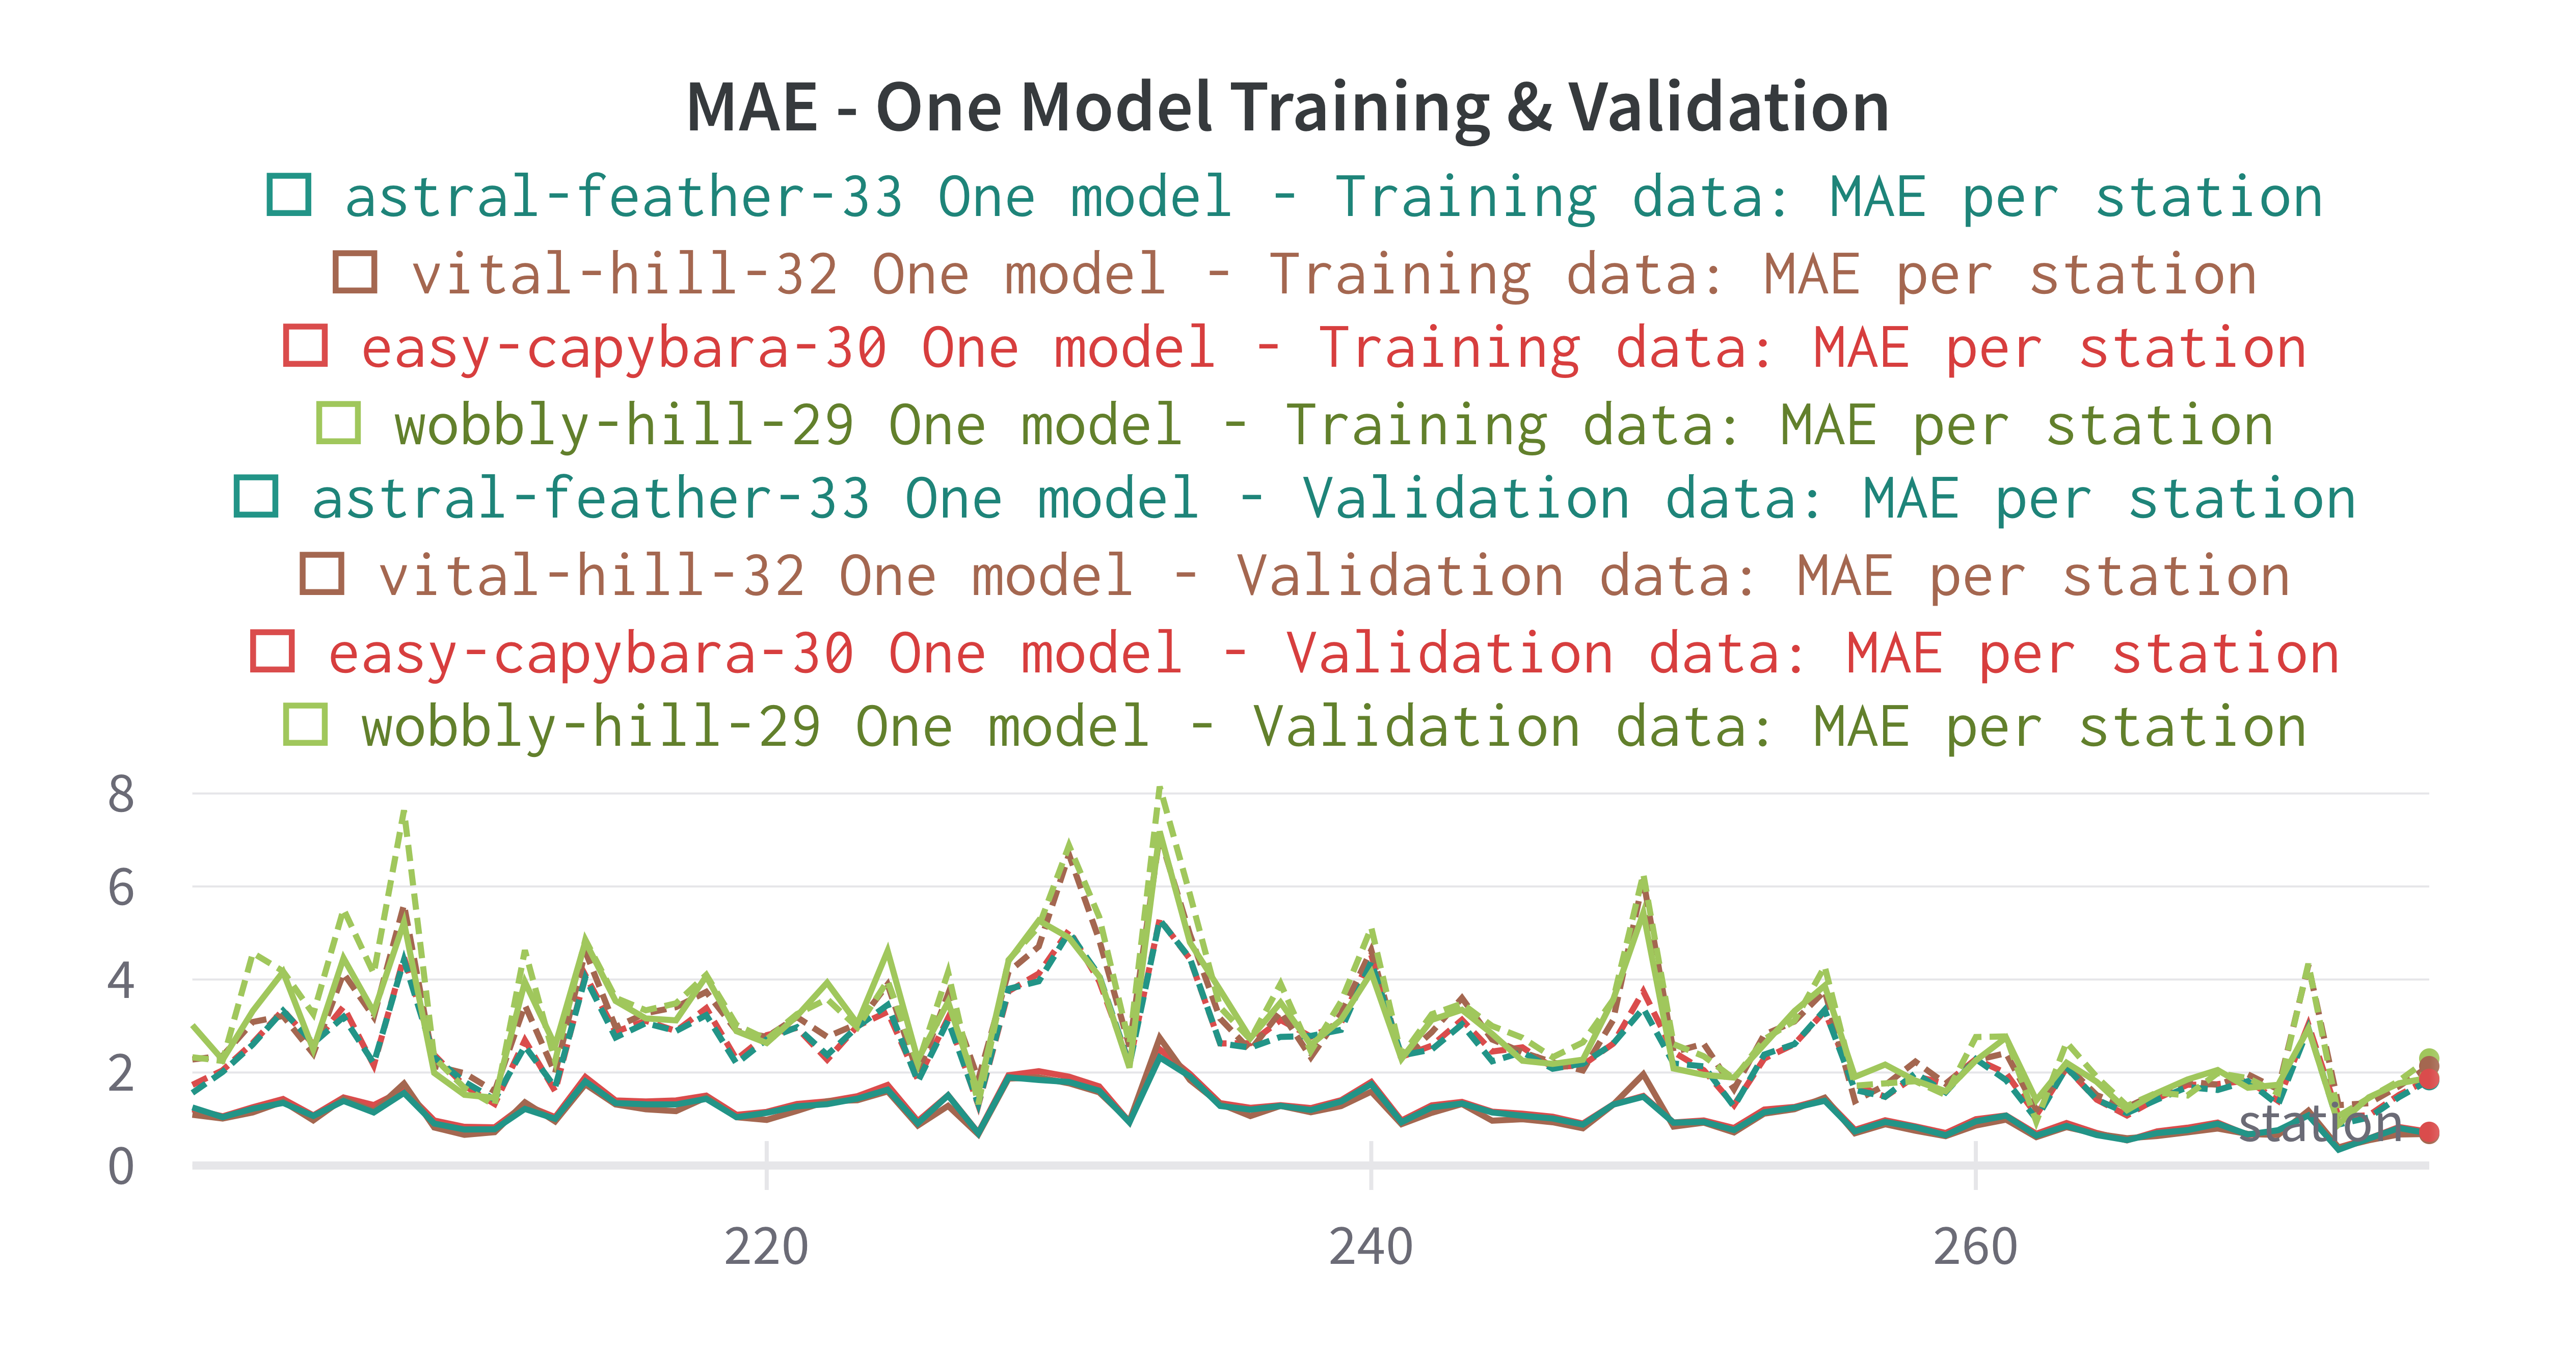
\includegraphics[width=0.5\textwidth]{mae-one-model-step3}
        \caption{MAE for Random Forest Regressor with more features for approach a) and b)}
        \label{fig:step3-mae}
    \end{figure}

    I also tried a few other feature combinations and they can be looked at in details on wandb. None of these outperformed
    the best ones described in more detail in this section. As expected temperature was not a good feature nor was just one
    of the bike profiles:
    \begin{itemize}
        \item \href{https://wandb.ai/idegen/mlp-2021/runs/2ft9d86n?workspace=user-idegen}{dauntless-wood-36} -
        features: station, bikes\_3h\_ago, numDocks, weekhour, isHoliday, full\_profile\_bikes, full\_profile\_3h\_diff\_bikes
        \item \href{https://wandb.ai/idegen/mlp-2021/runs/1shg15eq?workspace=user-idegen}{soft-deluge-35} -
        features: station, bikes\_3h\_ago, numDocks, weekhour, isHoliday, temperature.C
        \item \href{https://wandb.ai/idegen/mlp-2021/runs/1tsar458?workspace=user-idegen}{driven-cosmos-34} -
        features: station, bikes\_3h\_ago, numDocks, weekhour, isHoliday, airPressure.mb
    \end{itemize}


    \subsubsection*{\nameref{itm:phase1-step4}}

    In total I ran 6 different sweeps all for the Random Forest Model. For sweep 4-6 I also changed the features used which
    had by fare the most important impact on MAE. All the sweeps and their results are logged on wandb:
    \begin{itemize}
        \item \href{https://wandb.ai/idegen/mlp-2021/sweeps/ylvvcigm?workspace=user-idegen}{Random Forest Regressor Sweep 1}
        \item \href{https://wandb.ai/idegen/mlp-2021/sweeps/79bi8rgn?workspace=user-idegen}{Random Forest Regressor Sweep 2}
        \item \href{https://wandb.ai/idegen/mlp-2021/sweeps/42mzcyb3?workspace=user-idegen}{Random Forest Regressor Sweep 3}
        \item \href{https://wandb.ai/idegen/mlp-2021/sweeps/rrpaocle?workspace=user-idegen}{Random Forest Regressor Sweep 4}
        \item \href{https://wandb.ai/idegen/mlp-2021/sweeps/au3spnyx?workspace=user-idegen}{Random Forest Regressor Sweep 5}
        \item \href{https://wandb.ai/idegen/mlp-2021/sweeps/lc68mqc3?workspace=user-idegen}{Random Forest Regressor Sweep 6}
    \end{itemize}

    \begin{figure}[h]
        \centering
        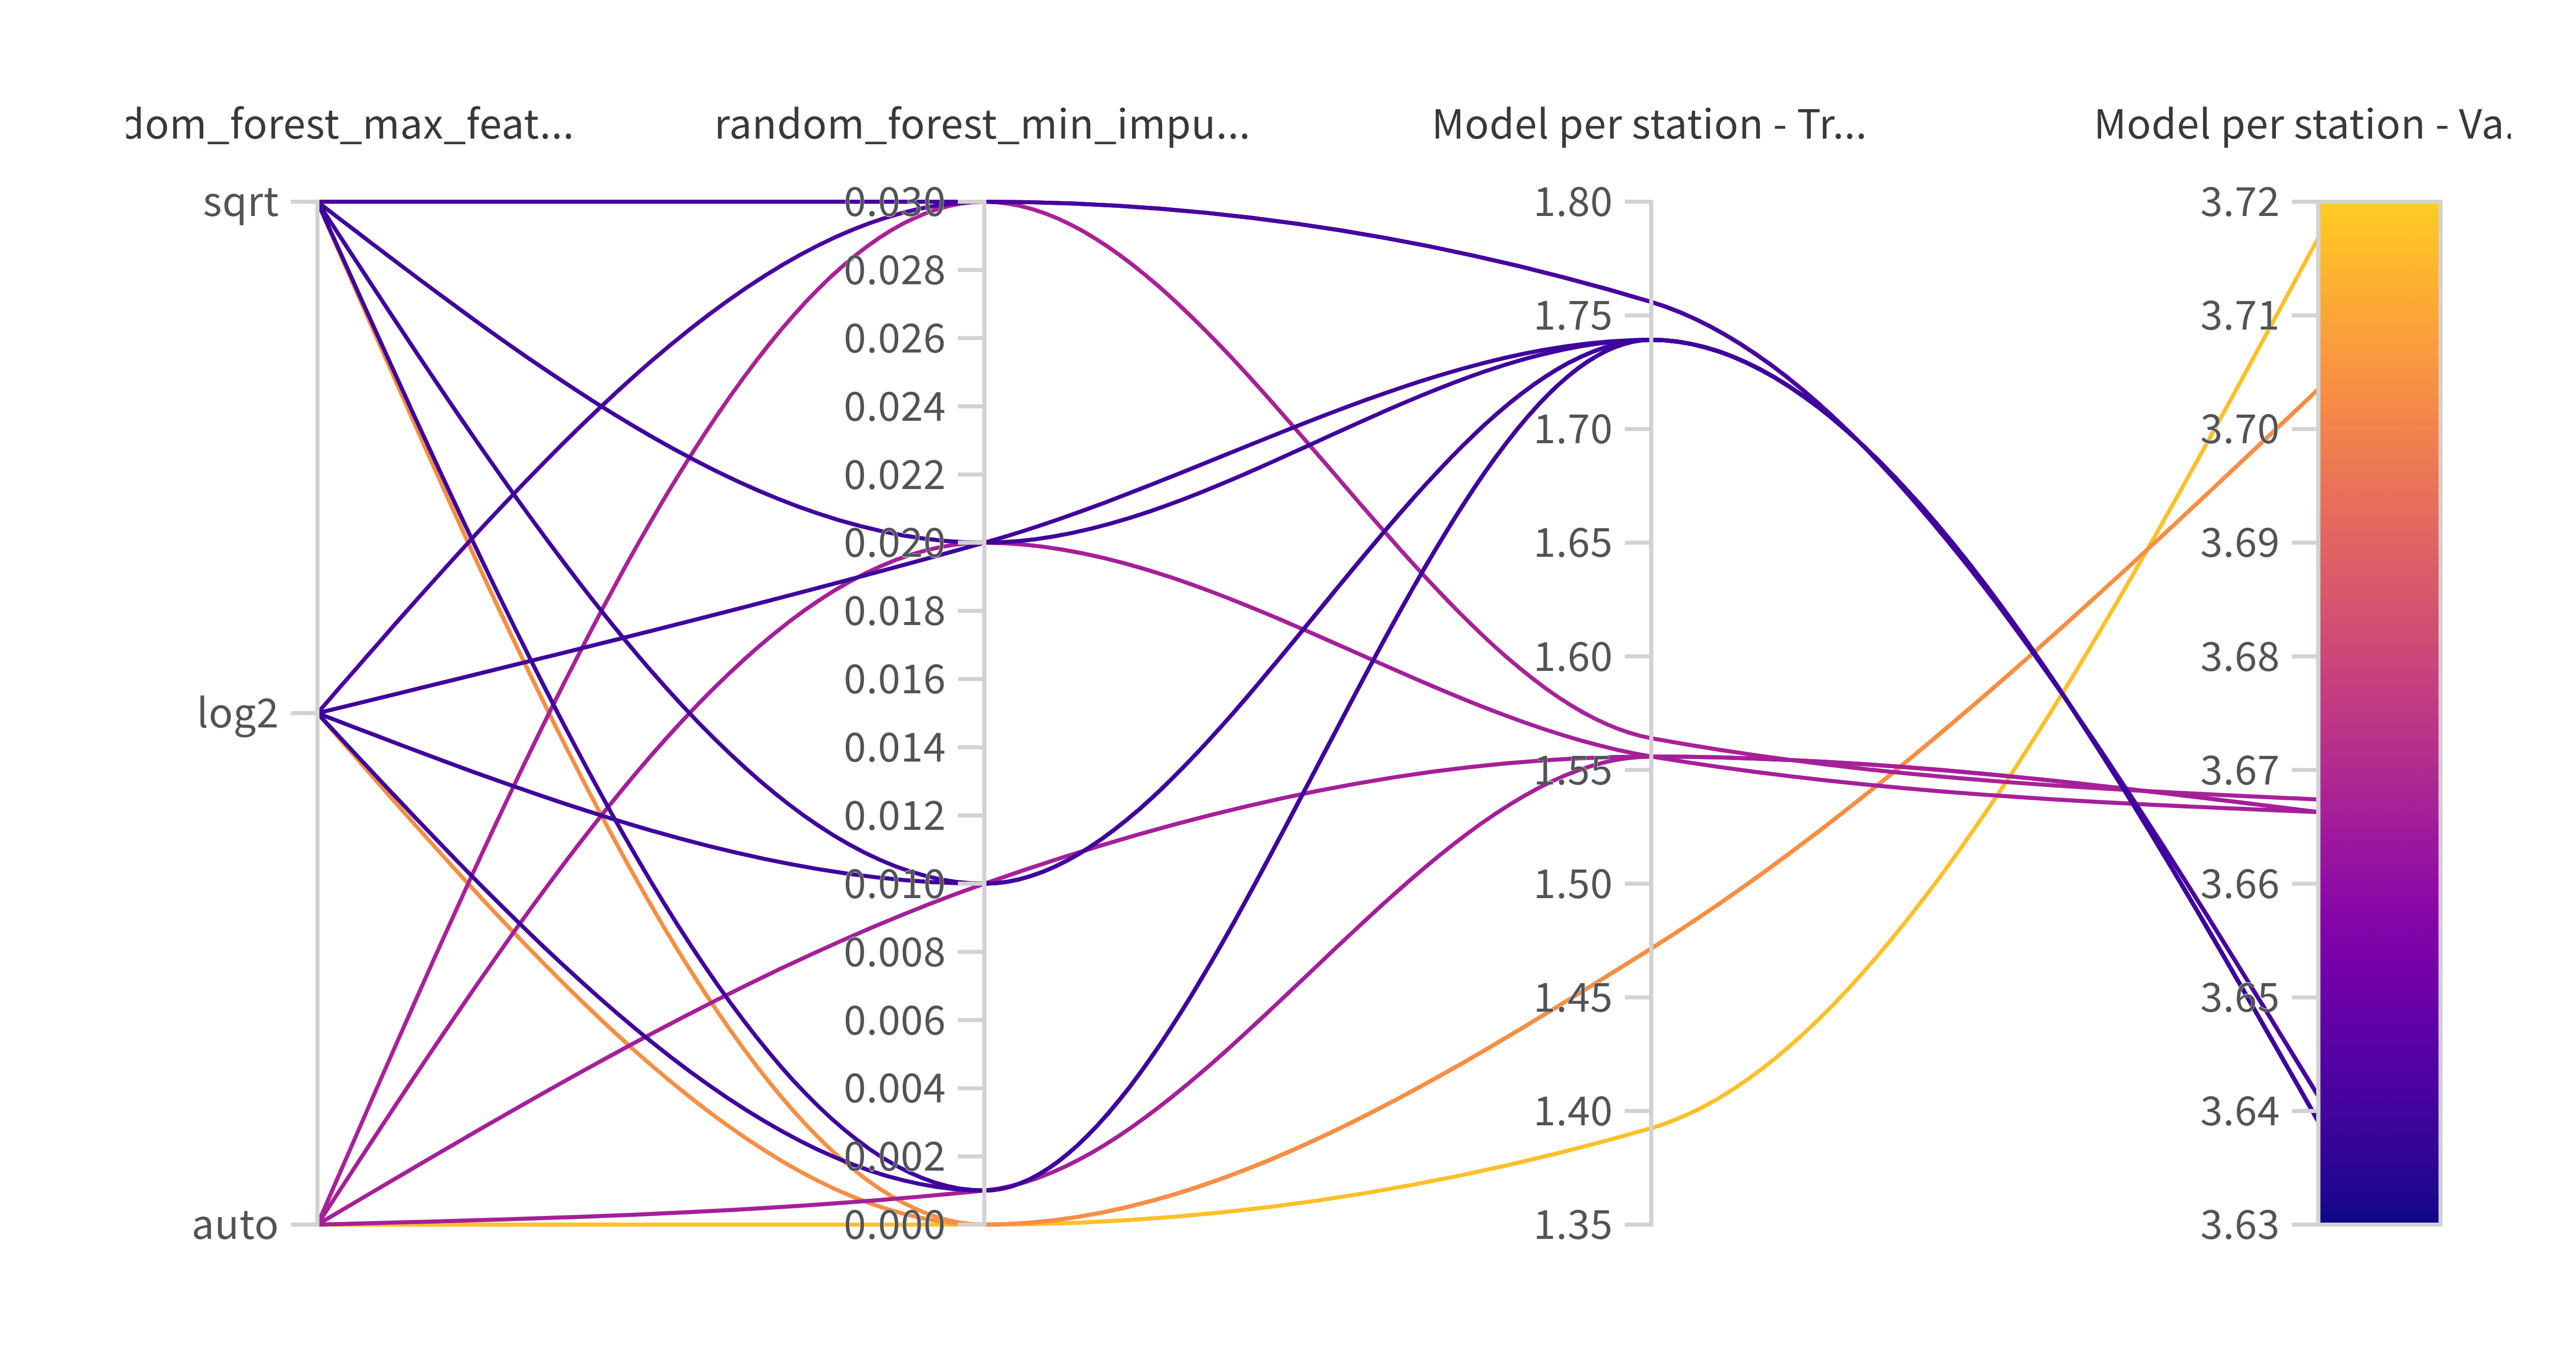
\includegraphics[width=0.8\textwidth]{randomforest-sweep3}
        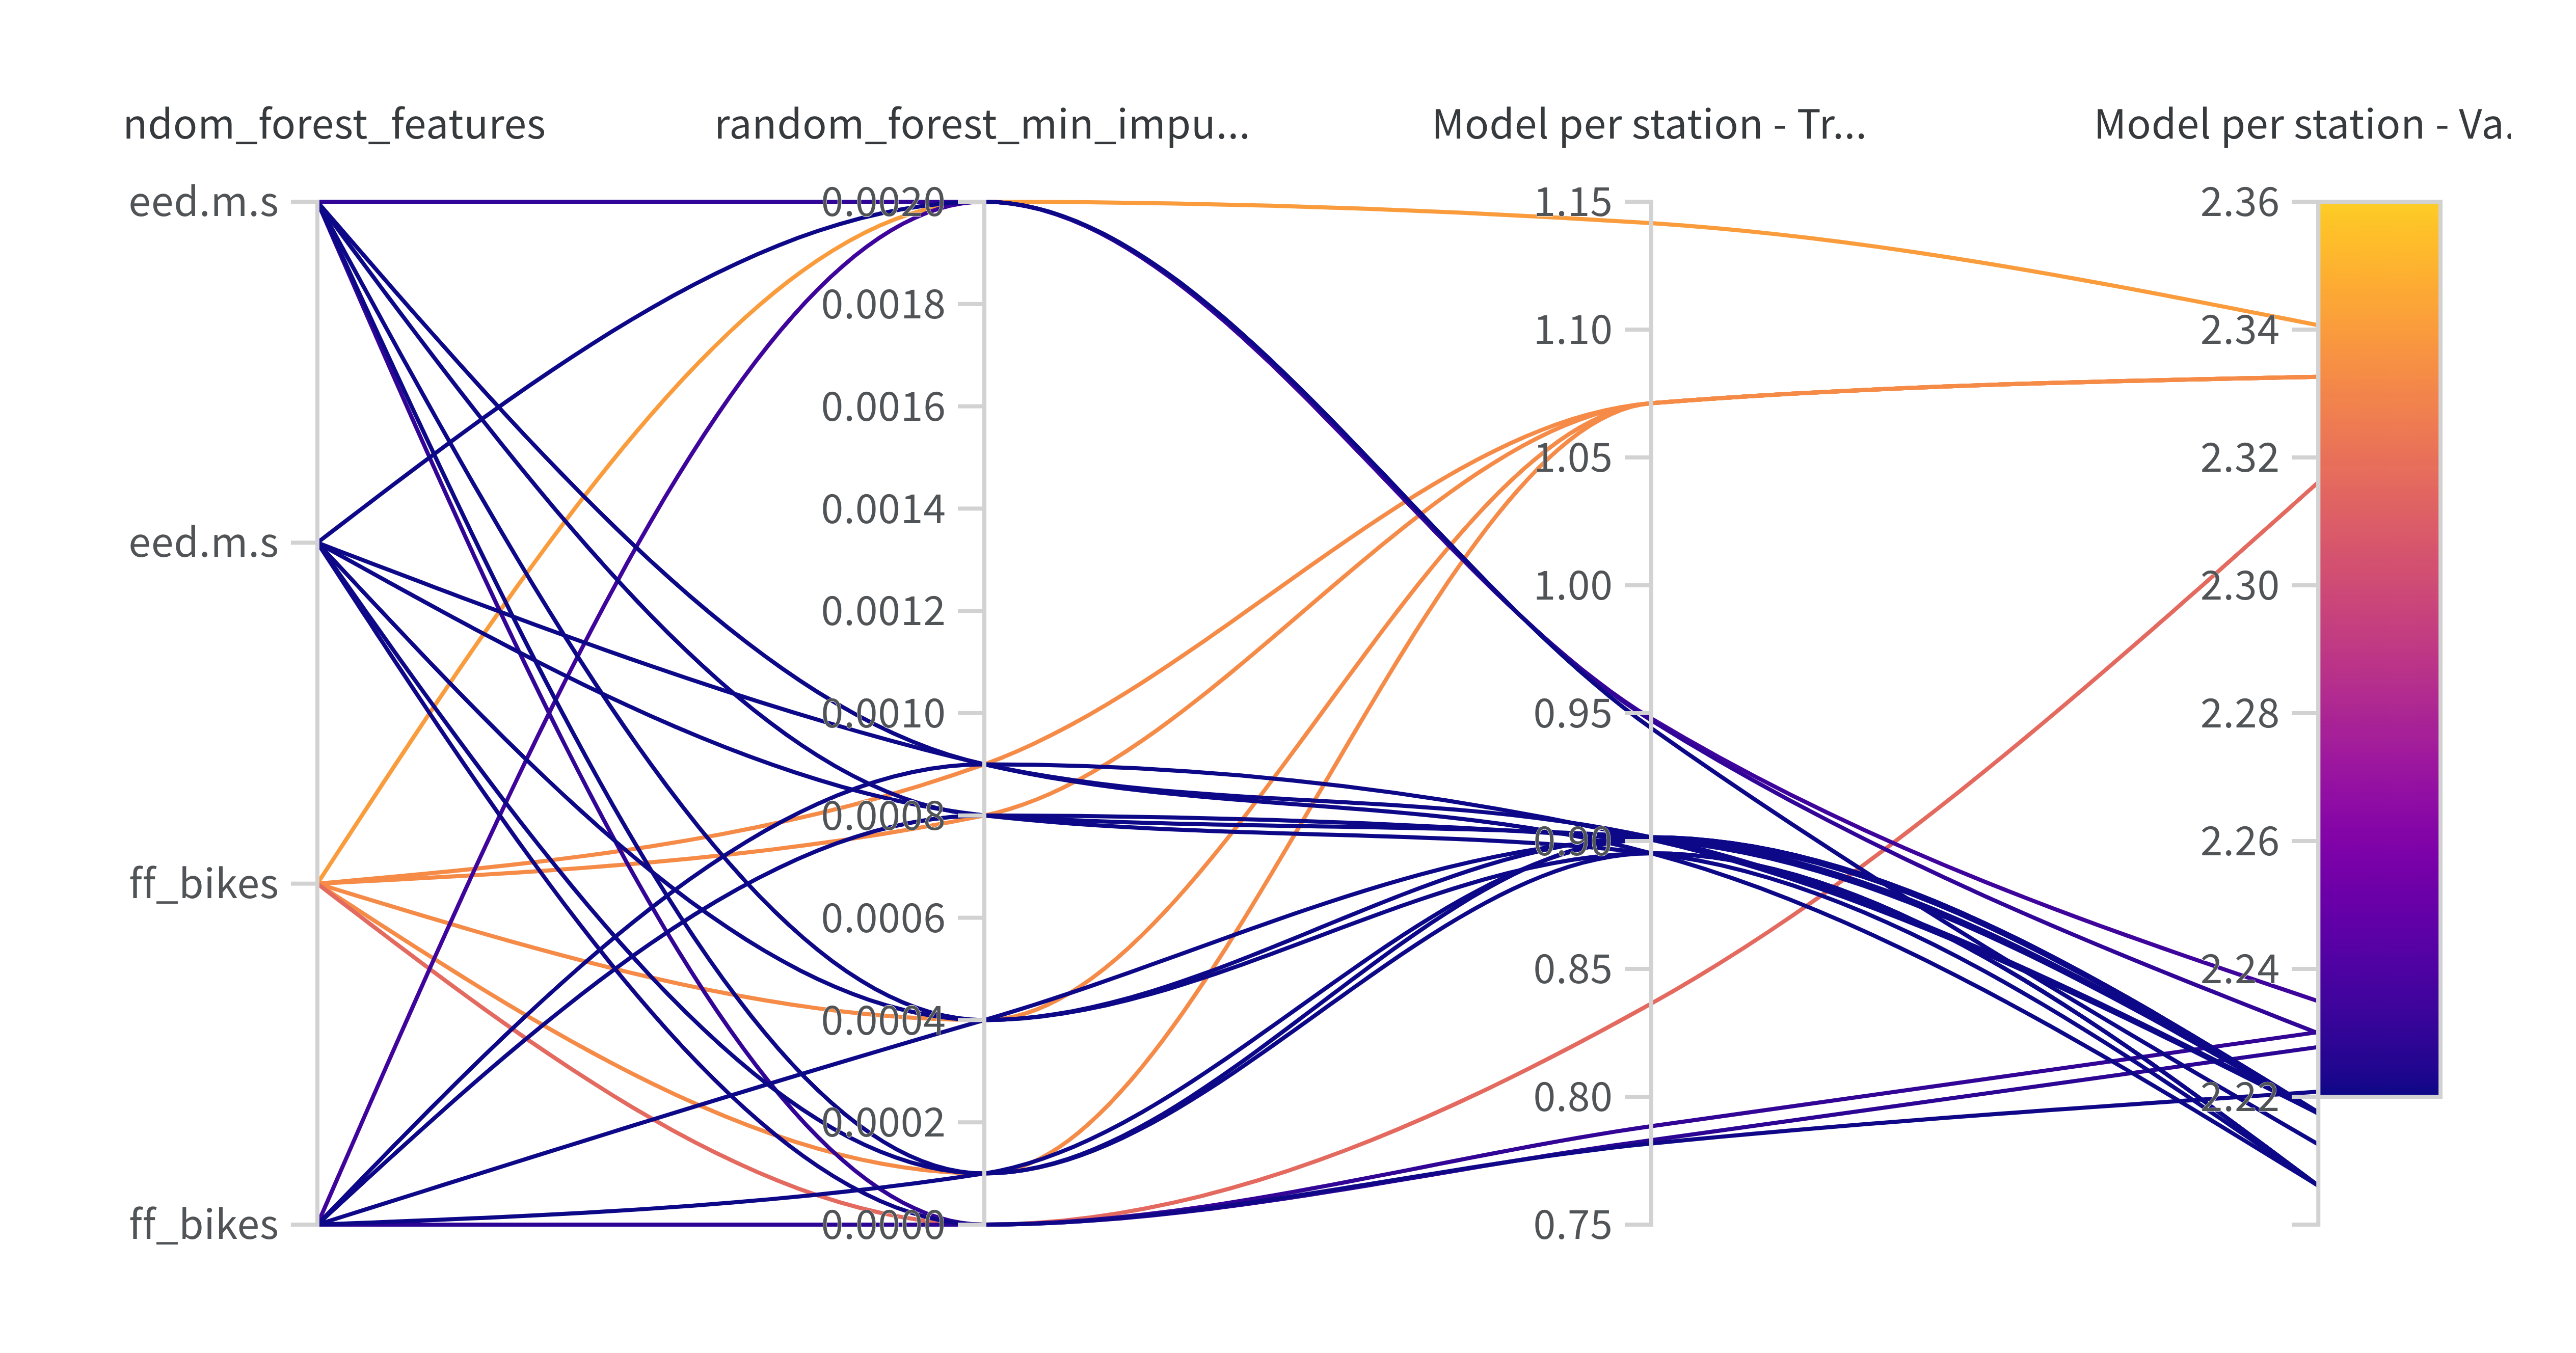
\includegraphics[width=0.8\textwidth]{random-forest-sweep6}
        \caption{Parallel Coordinates Graph for Random Forest Sweep 3 (top) and 6 (bottom). The right hand sight is the
        validation MAE the second last column the training dataset MAE. The labels are too long to download but the
        full interactive graphs can be investigated on wandb.}
        \label{fig:sweep3and6RandomForest}
    \end{figure}

    Using the best performing features from \nameref{itm:phase1-step3}:station, bikes\_3h\_ago, numDocks, weekhour, isHoliday
    only varying the hyperparameters resulted in the lowest MAE for the training dataset of 1.392. However that run at
    a big validation dataset MAE of 3.717. The lowest validation dataset MAE was 3.639 for which the training dataset
    MAE was 1.739. In short this was worse than what I had achieved with varying features in \nameref{itm:phase1-step3}.
    The best performing features combination was: station, bikes\_3h\_ago, numDocks, weekhour, isHoliday, full\_profile\_bikes,
    full\_profile\_3h\_diff\_bikes, airPressure.mb, relHumidity.HR, windMeanSpeed.m.s. This achieved a training MAE of 0.89
    and a validation MAE of 2.206. Note that these MAE are only on a part of the dataset and cannot be directly compared
    to the full runs.

    For the best sweep result I also ran the full experiment which resulted in the
    \href{https://wandb.ai/idegen/mlp-2021/runs/2kmp7odq?workspace=user-idegen}{floral-pine-419} experiment. Figure \ref{fig:sweep3and6RandomForest}
    shows the MAE per station for this experiment. The overall training MAE was 0.9 and the overall validation MAE was
    2.21. It scored 2.83 on the test dataset which was a slight improvement from the easy-capybara-30 experiment.

    \begin{figure}[h]
        \centering
        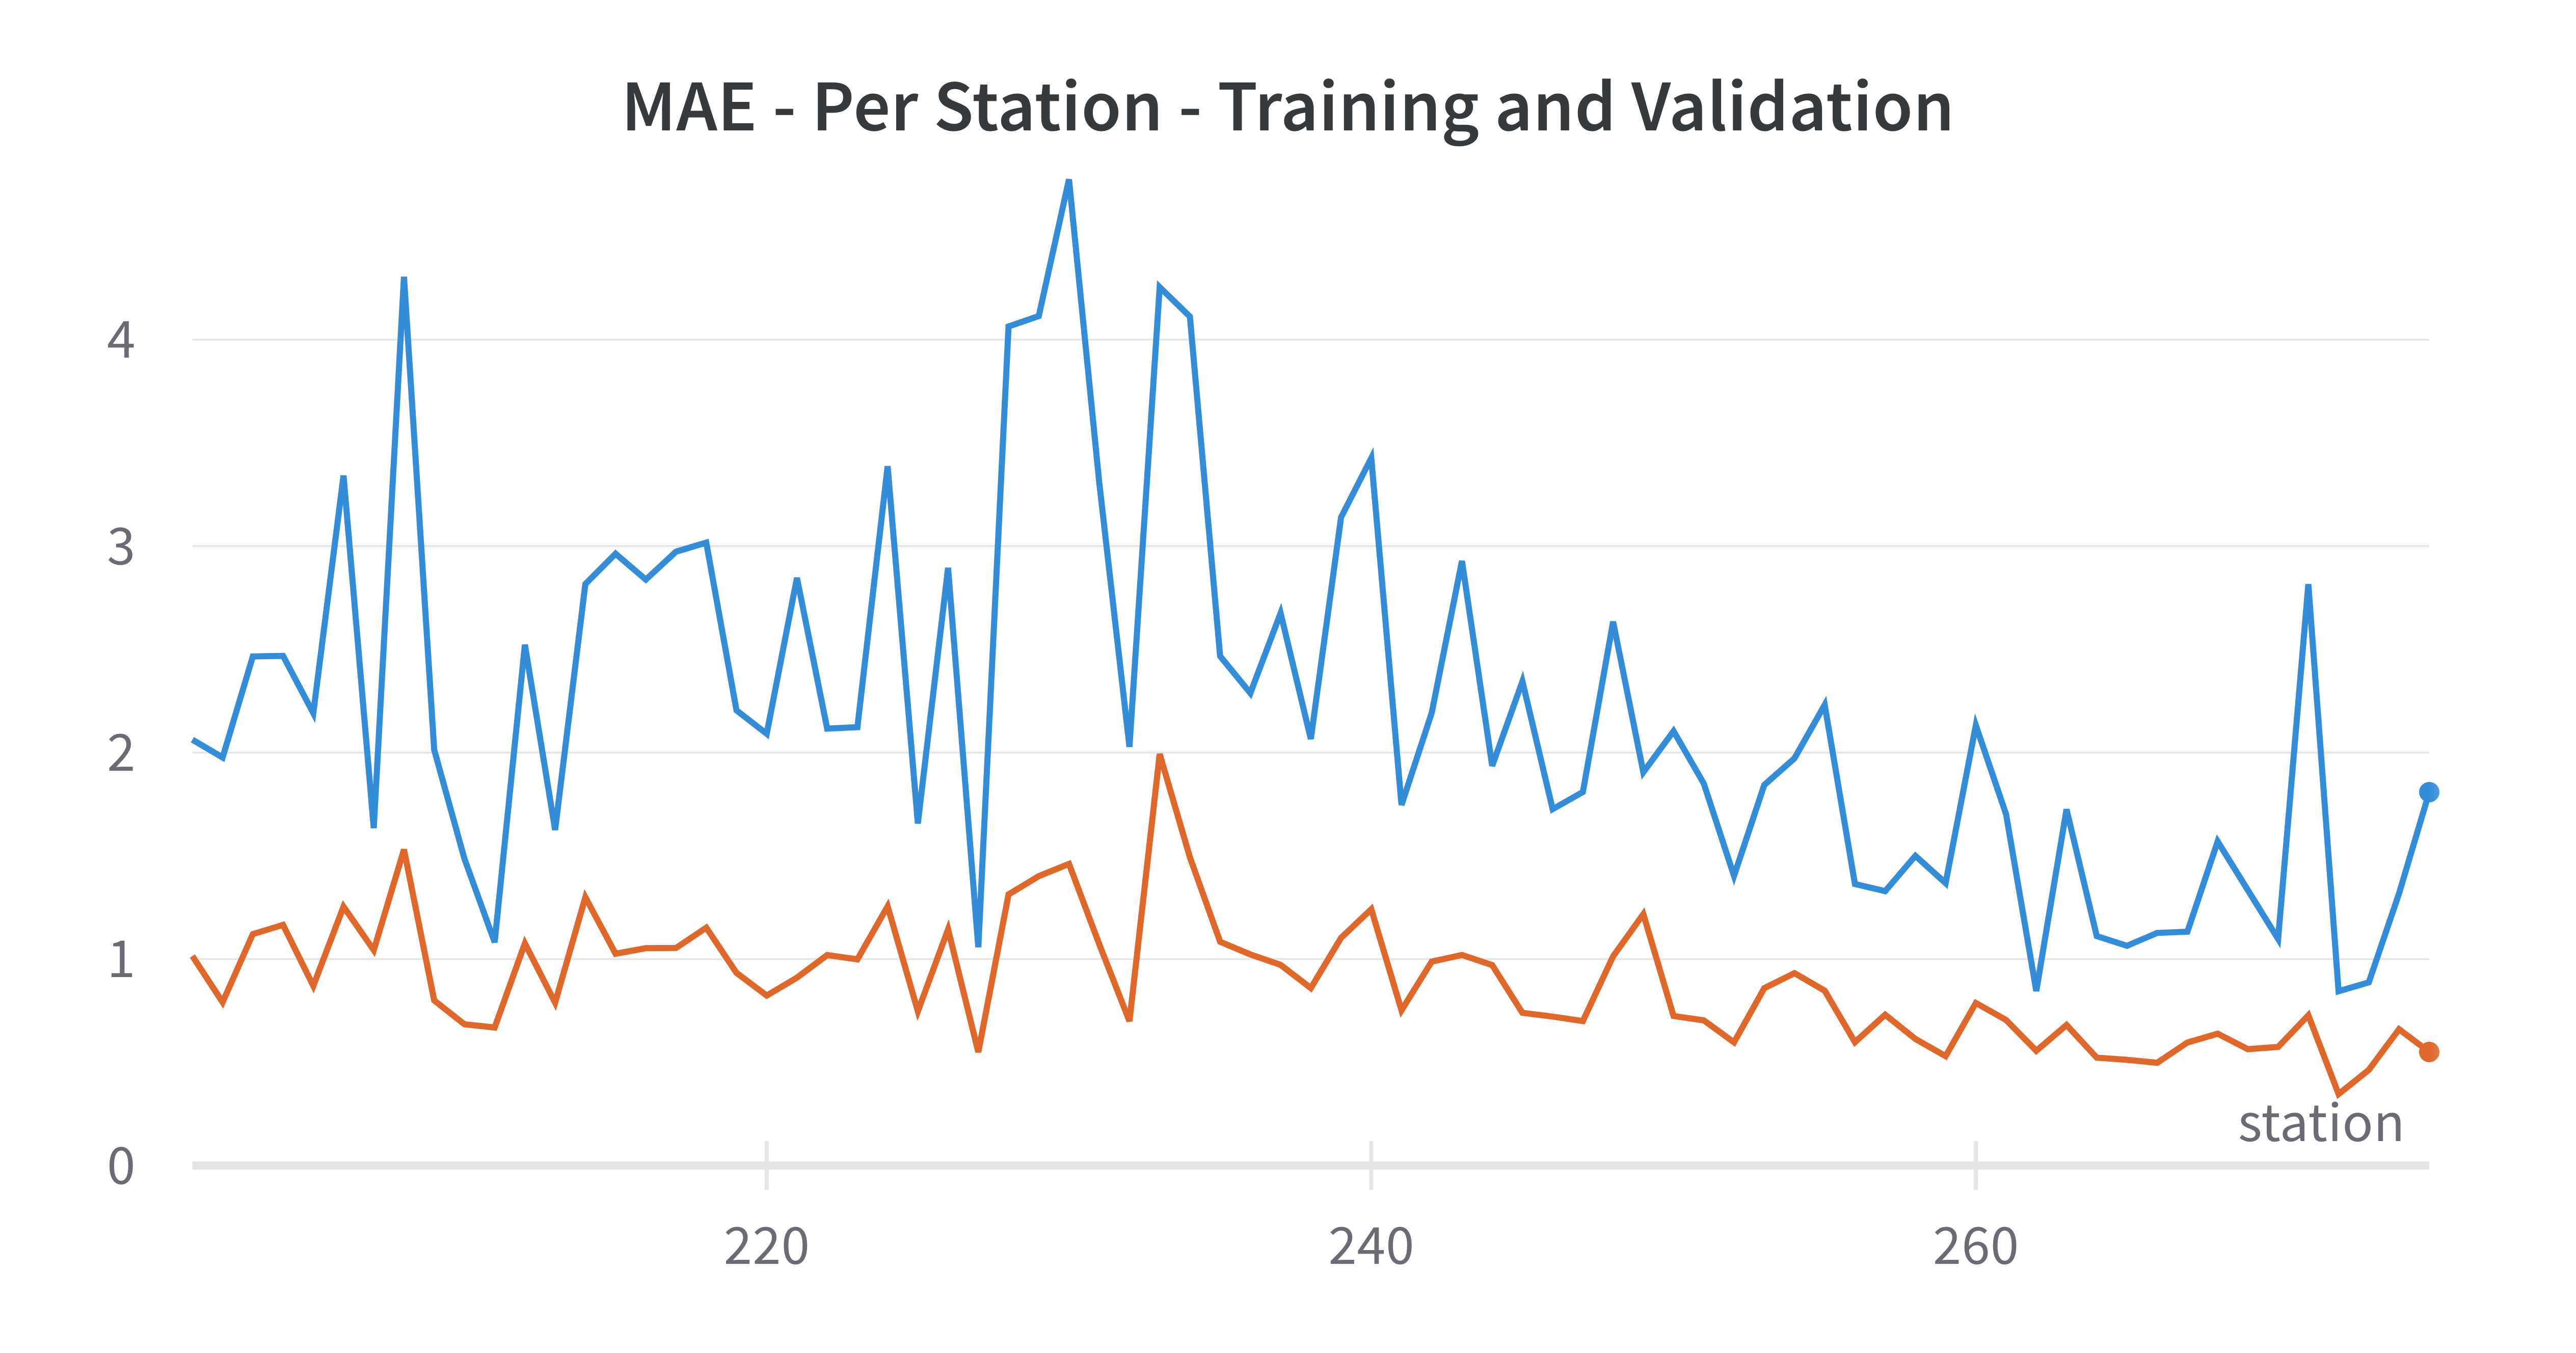
\includegraphics[width=0.6\textwidth]{floral-pine}
        \caption{Training and Validation dataset MAE for floral-pine experiment}
        \label{fig:floral-pine}
    \end{figure}

    The experiment with a Multilayer Perceptron Regresseor in it's default configuration and using the features: bikes\_3h\_ago,
    full\_profile\_bikes, full\_profile\_3h\_diff\_bikes, short\_profile\_bikes, short\_profile\_3h\_diff\_bikes achieved
    comparable MAEs: For the training dataset 2.498 and for the validation training set 2.67 and a surprising 2.41 on the test dataset,
    see experiment \href{https://wandb.ai/idegen/mlp-2021/runs/1of4938t?workspace=user-idegen}{clean-sunset-573} for all the details.
    While these MAE are not a significant improvement, the gap between the training and validation dataset is significantly
    smaller, see figure \ref{fig:clean-sunset}.

    \begin{figure}[h]
        \centering
        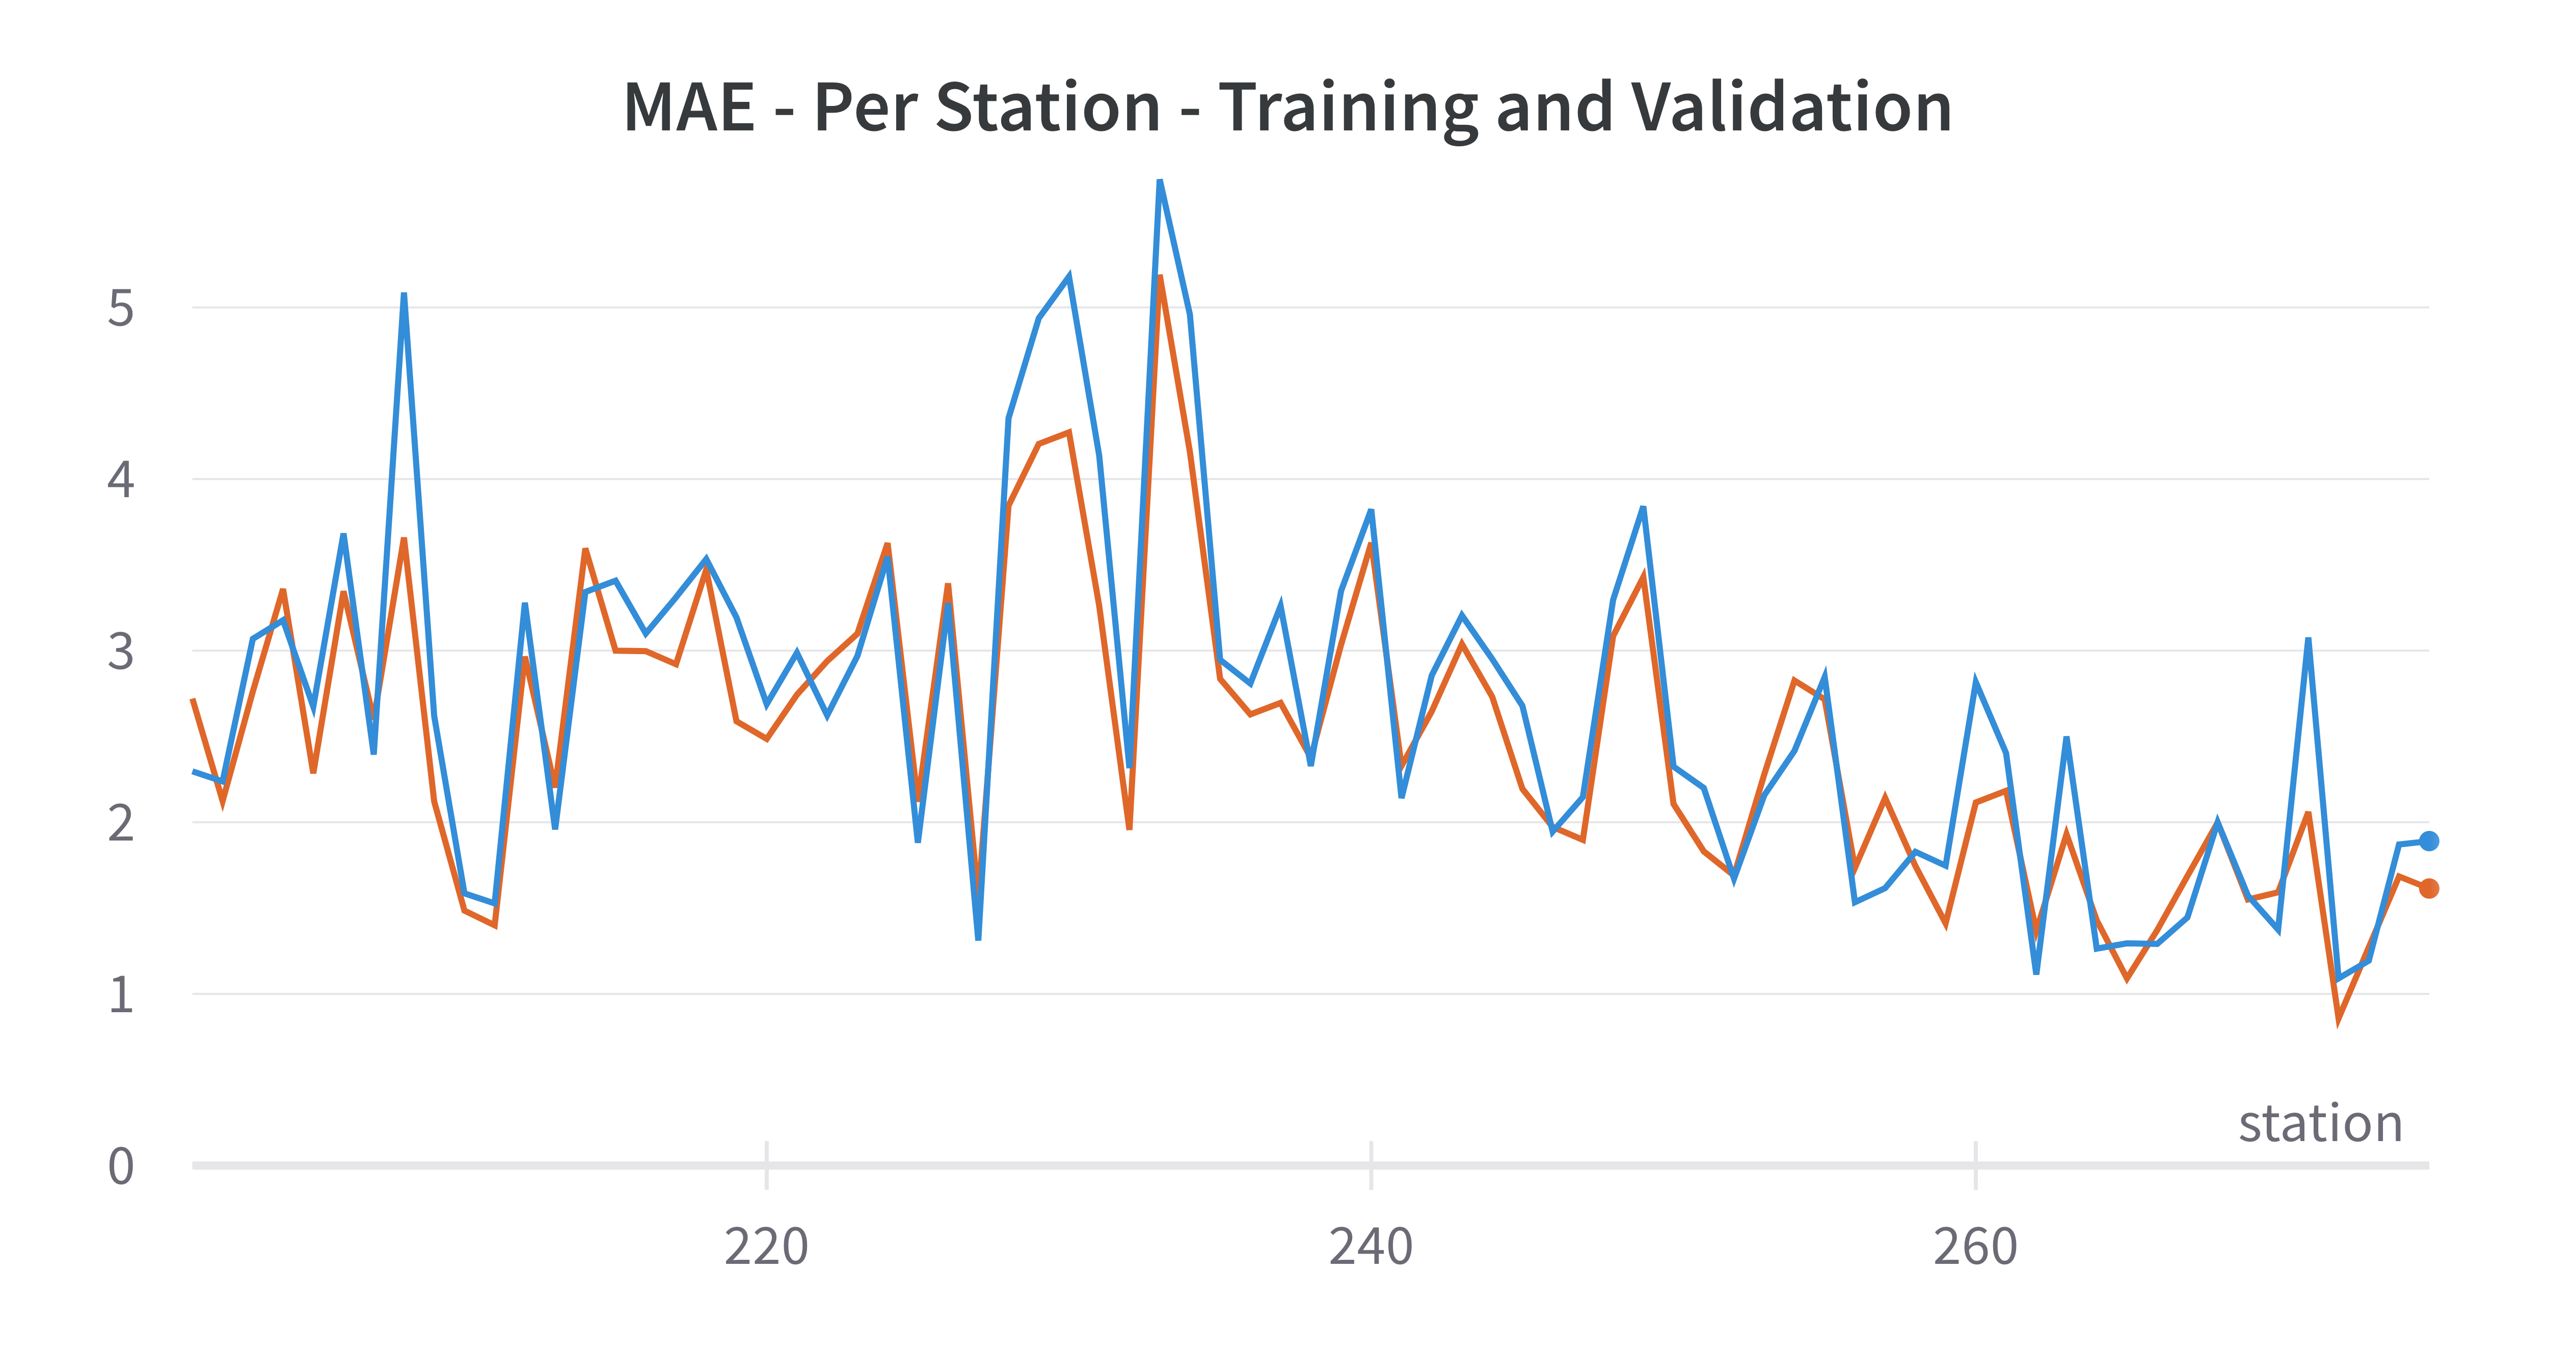
\includegraphics[width=0.4\textwidth]{model-per-station-clean-sunset}\hfill
        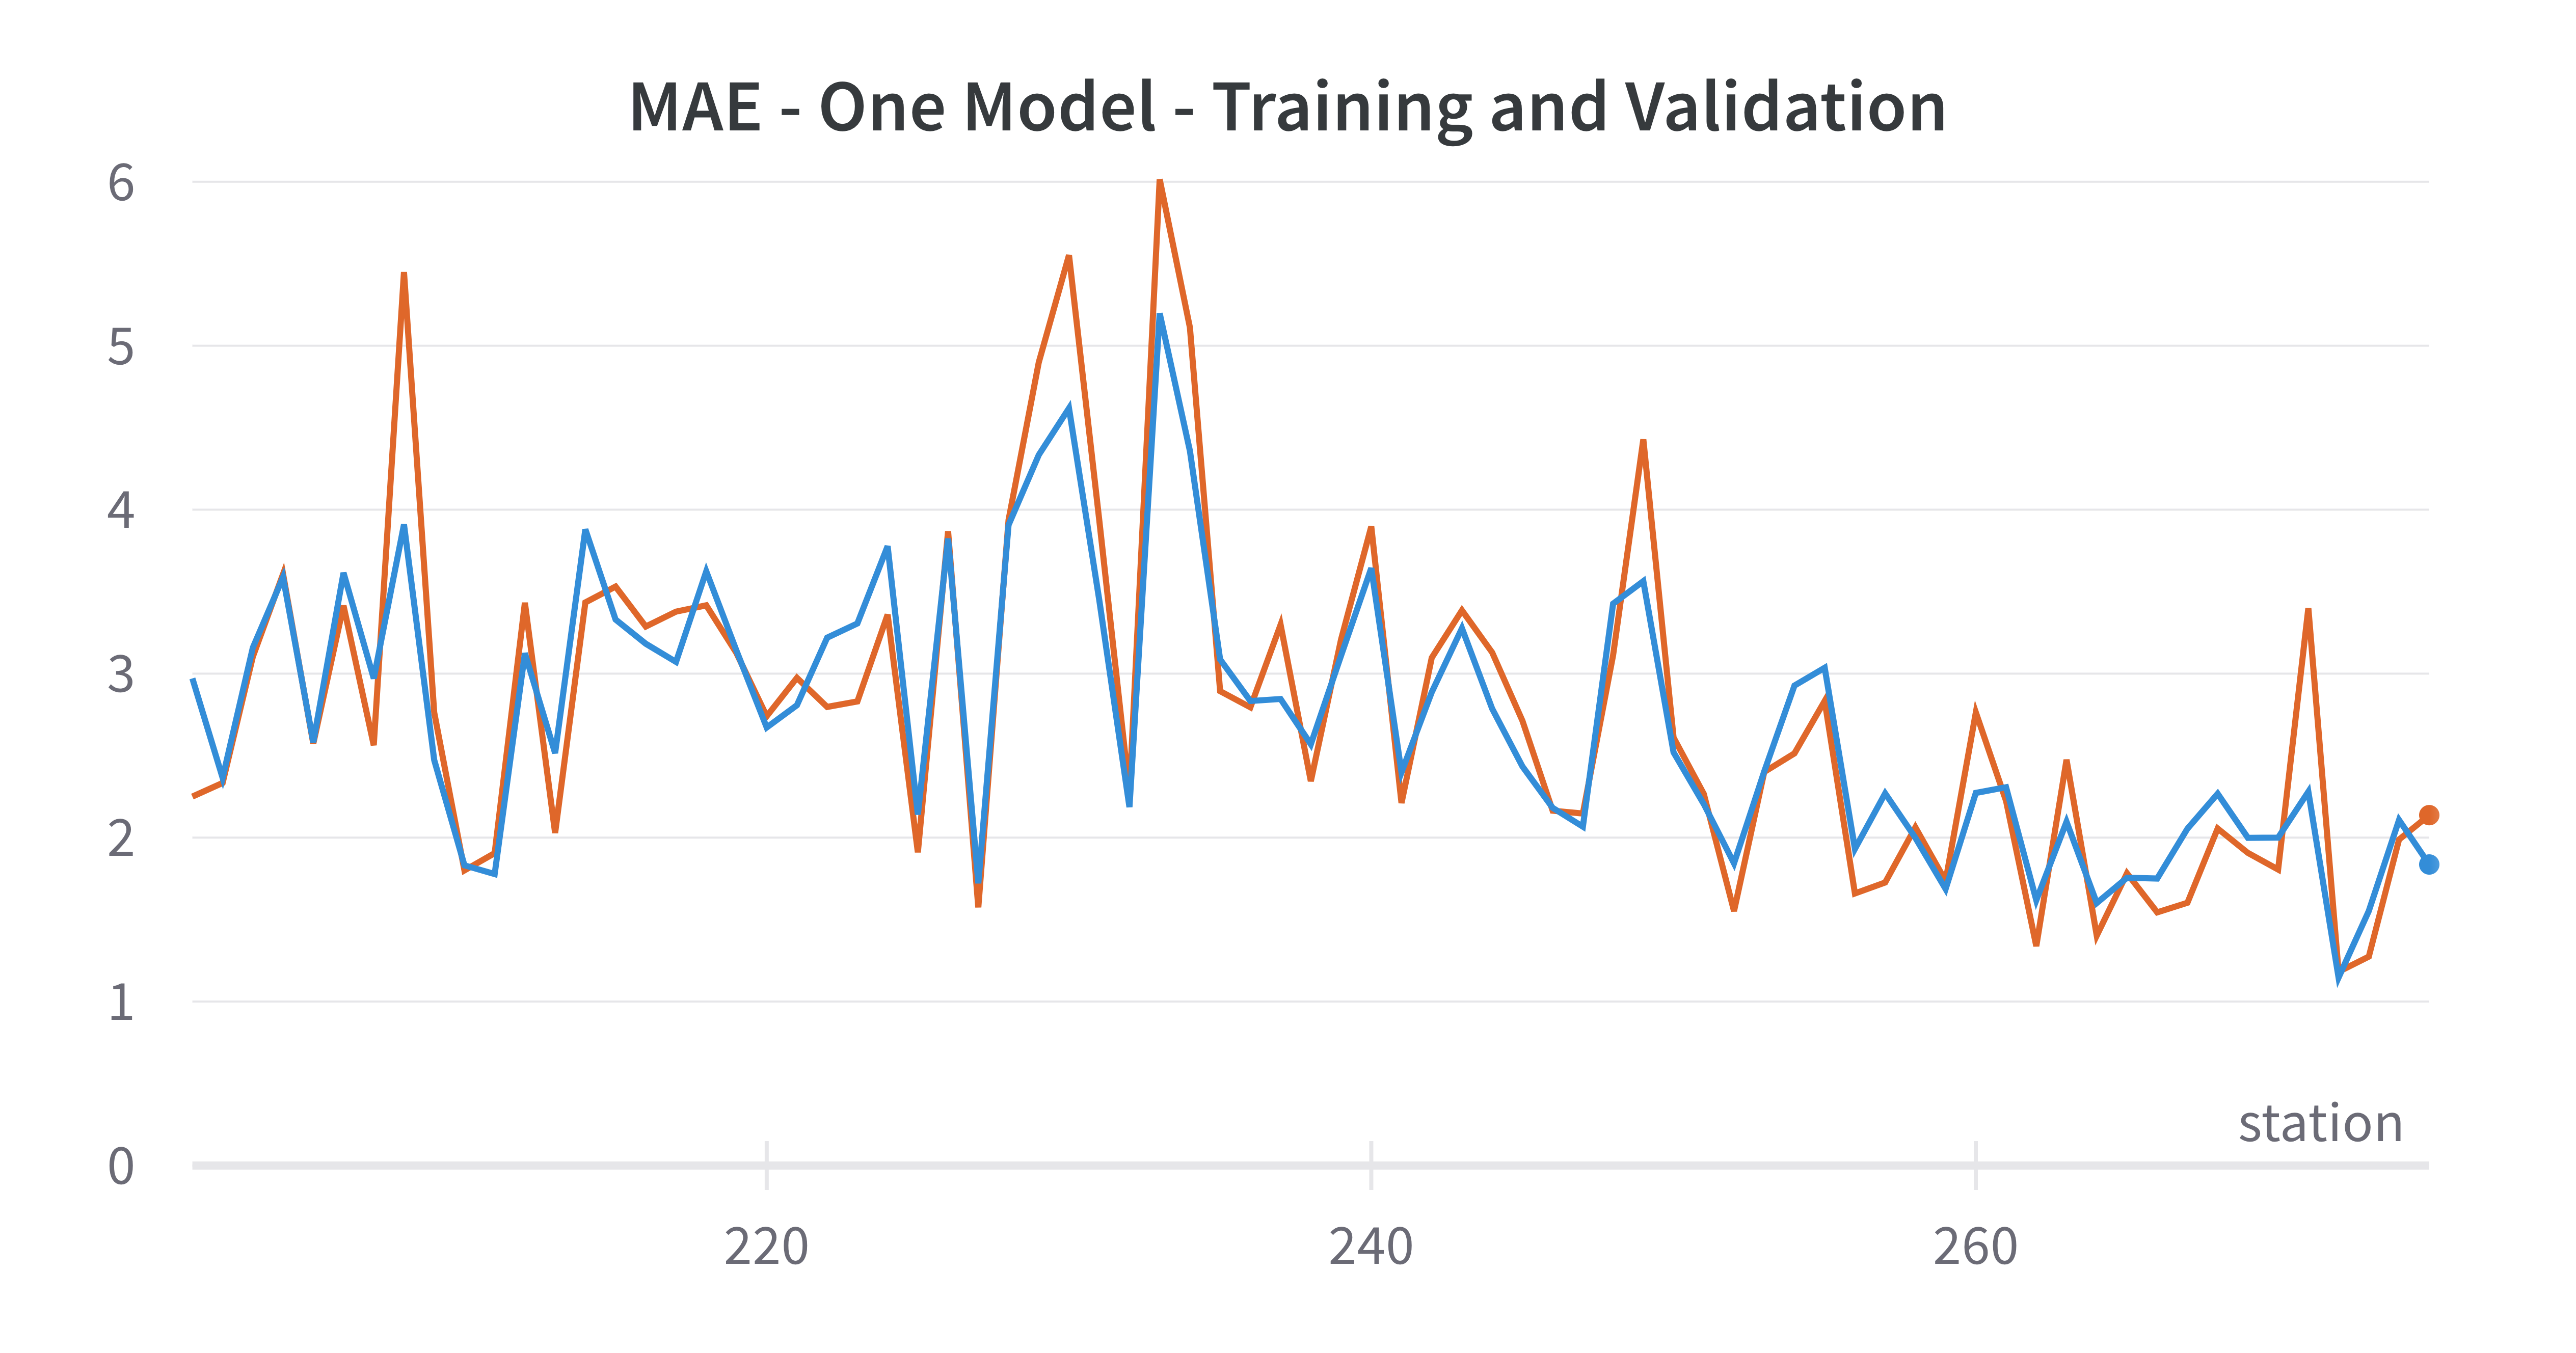
\includegraphics[width=0.4\textwidth]{onemodel-clean-sunset}
        \caption{Training and Validation MAE for the Multilayer Perceptron Regressor - clean-sunset-573}
        \label{fig:clean-sunset}
    \end{figure}

    \subsection*{\nameref{phs:two}}
    The results for predicting bikes for station 201-275 using solely the pretrained models for station 1-200 can be
    seen in experiment \href{https://wandb.ai/idegen/mlp-2021/runs/3rs1cuxc?workspace=user-idegen}{whole-rain-575}. Choosing
    the pretrained model which results in the lowest MAE on the training dataset results in an MAE for the training dataset of 2.569
    and an MAE for the validation dataset of 2.646 which is lower than the MAE achieved for the untuned Multilayer Perceptron,
    see figure \ref{fig:pre-trained-model}.

    \begin{figure}[h]
        \centering
        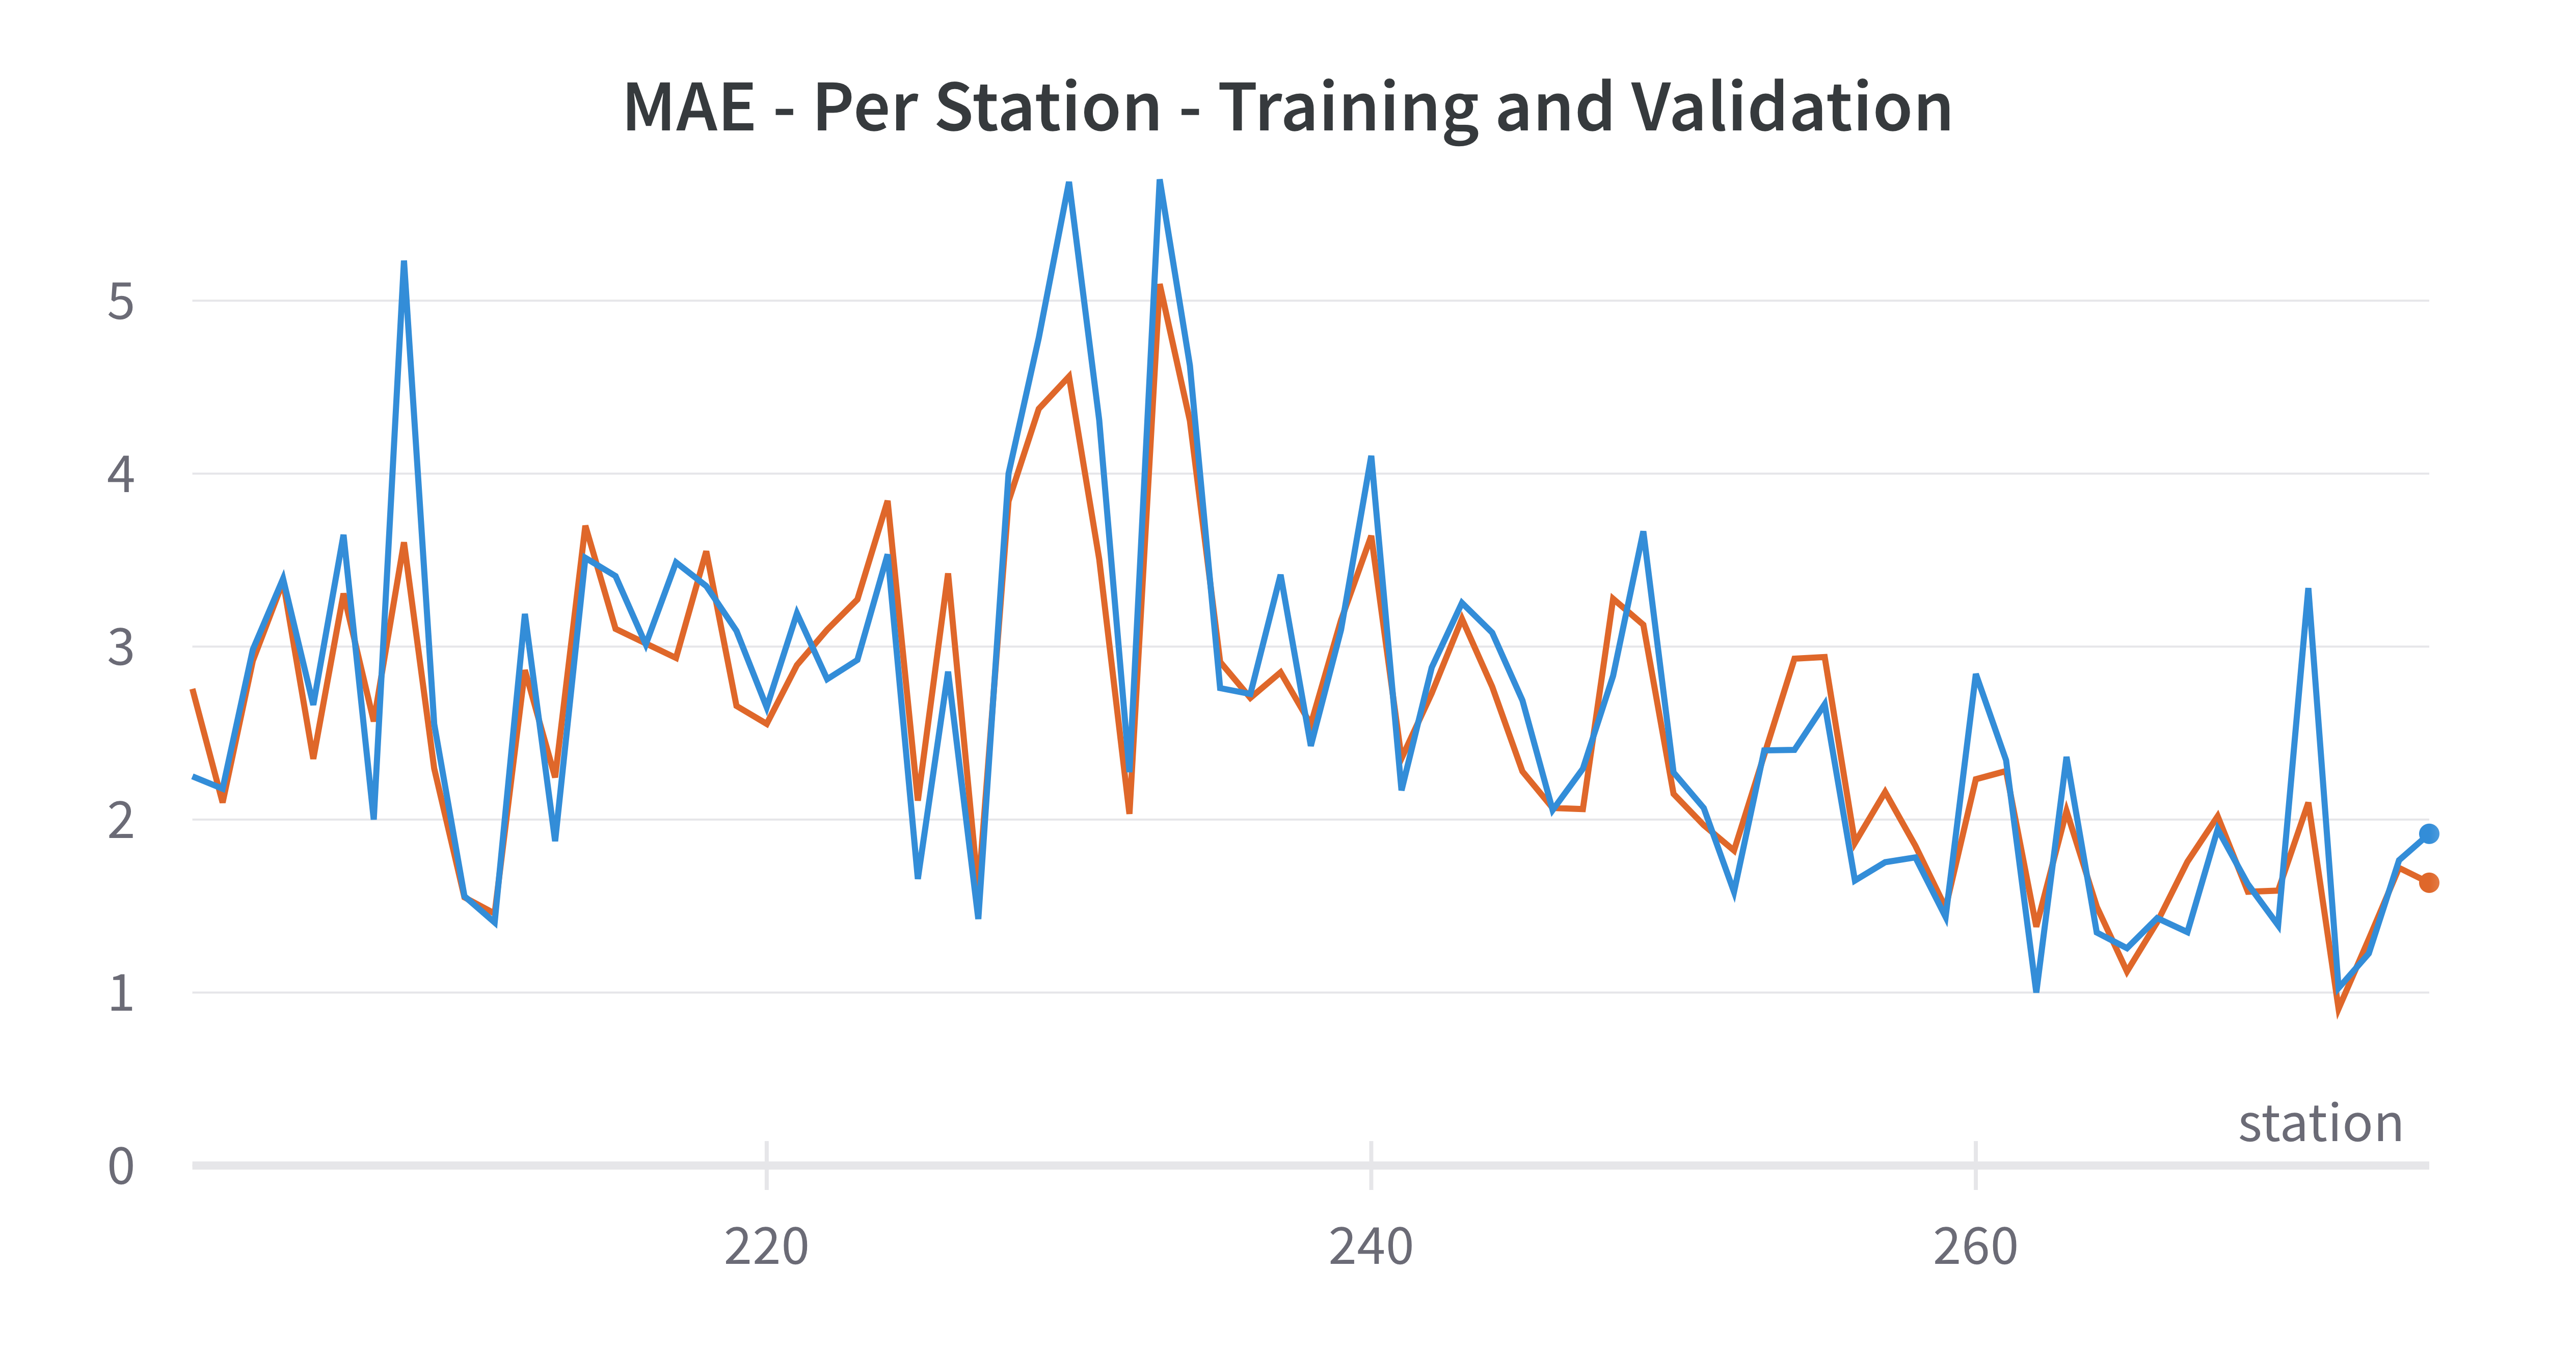
\includegraphics[width=0.6\textwidth]{pretrained-model}
        \caption{Training and Validation MAE for the best pretrained model - whole-rain-575}
        \label{fig:pre-trained-model}
    \end{figure}

    \subsection*{\nameref{phs:three}}

    The result for the untuned combination of best pretrained model and multilayer perceptron for each station can be seen
    in experiment \href{https://wandb.ai/idegen/mlp-2021/runs/ogsyvkqu?workspace=user-idegen}{young-dragon-628}. The
    MAE for the training dataset was 2.485 and for the validation dataset 2.617 which is an improvement both on the pretrained model
    as well as the multilayer perceptron regressor.

    I ran a total of 7 sweeps to tune the parameters for the \href{https://wandb.ai/idegen/mlp-2021/sweeps?workspace=user-idegen}{multilayer preceptron regressor}.
    Figure shows a multicoordinate graph showing different architecture configurations and their impact on training and
    validation MAE, the interactive version can be found \href{https://wandb.ai/idegen/mlp-2021/sweeps/rughds30?workspace=user-idegen}{here}.
    I also ran sweeps that were trying out different features.

    \begin{figure}[h]
        \centering
        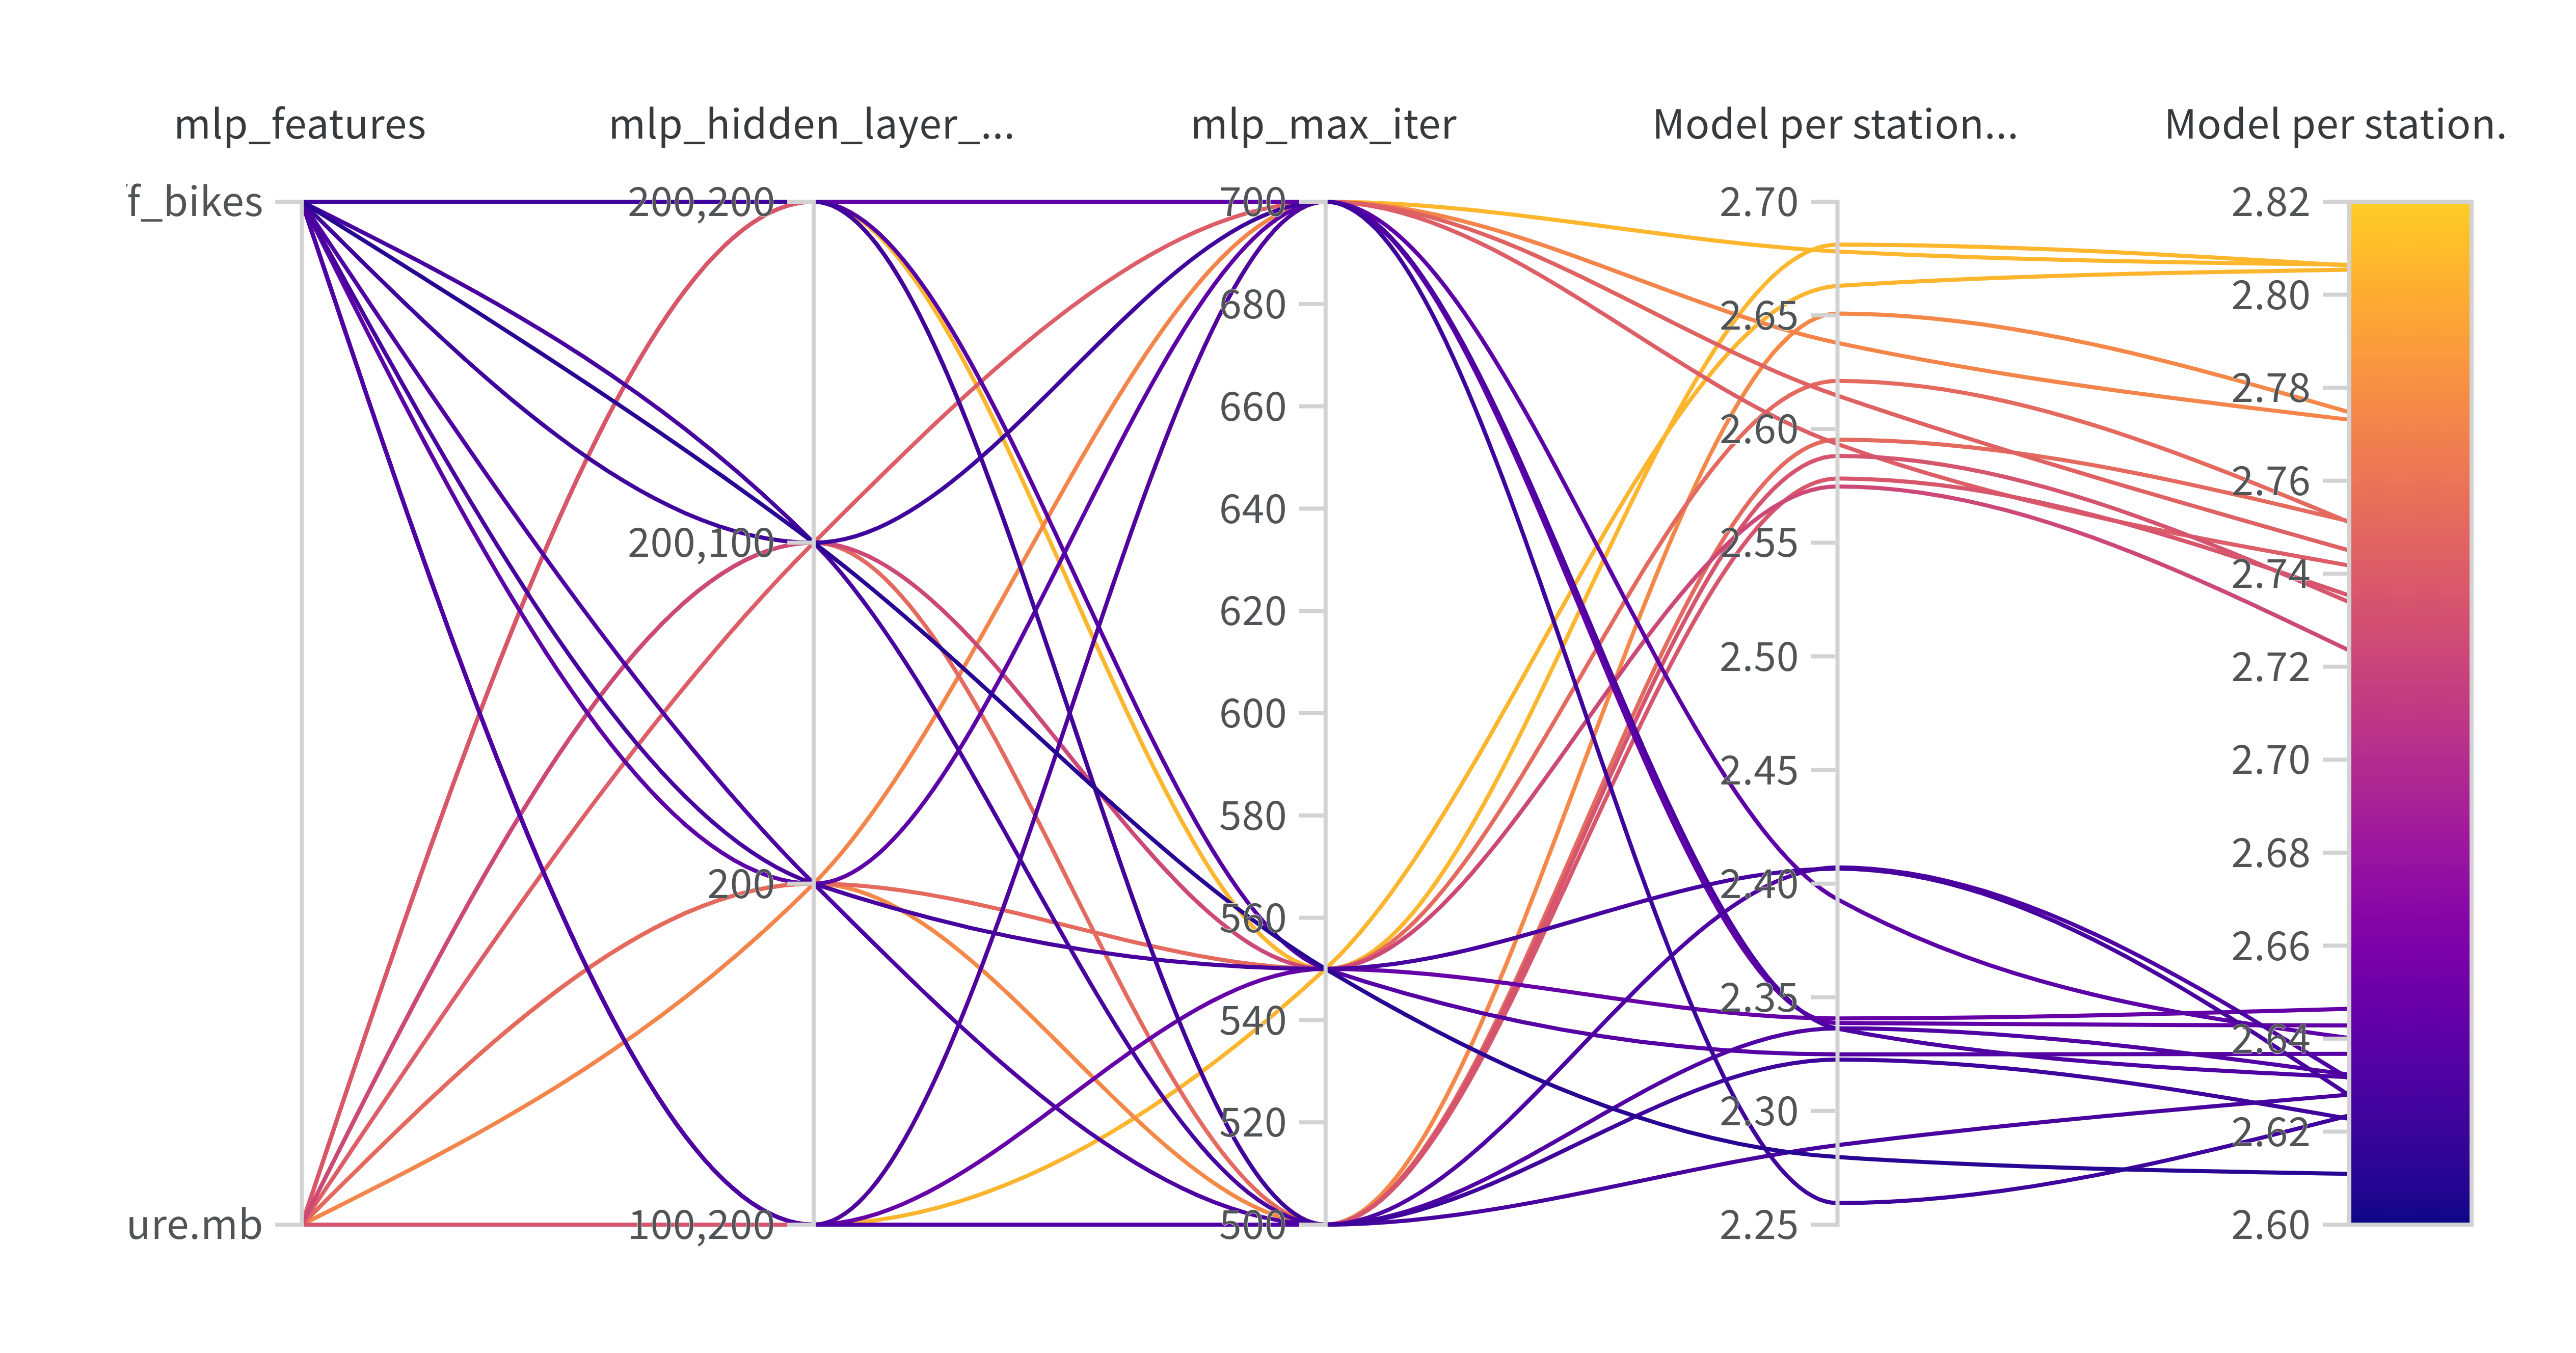
\includegraphics[width=0.8\textwidth]{mlp-sweep}
        \caption{Multiple coordinates graph for Multilayer Perceptron regessor sweep of diffeent architectures}
        \label{fig:mlp-sweep}
    \end{figure}

    Tuning the hyper parameters of the multilayer perceptron regressor further improved on this performance resulting
    in the best run achieved on Kaggle for the test dataset
    \href{https://wandb.ai/idegen/mlp-2021/runs/2w4l1irf?workspace=user-idegen}{worthy-dream-627}, table
    \ref{tbl:phase3}
    shows the result for the three best combined model expriments.

    \begin{table}[h]
        \begin{tabularx}{\textwidth}{|X|p{0.4\textwidth}|XXX|}
            \hline
            \multirow{2}{*}{Experiment name} &
            \multirow{2}{*}{Features} &
            \multicolumn{3}{l|}{a) Model per station} \\ \cline{3-5}
            &
            &
            \multicolumn{1}{l|}{Training} &
            \multicolumn{1}{l|}{Validation} &
            Test \\ \hline
            \href{https://wandb.ai/idegen/mlp-2021/runs/2w4l1irf?workspace=user-idegen}{fluent-morning-923} &
            weekhour, bikes\_3h\_ago, full\_profile\_bikes, full\_profile\_3h\_diff\_bikes, short\_profile\_bikes, short\_profile\_3h\_diff\_bikes &
            \multicolumn{1}{l|}{2.343} &
            \multicolumn{1}{l|}{2.545} &
            2.431 \\ \hline
            \href{https://wandb.ai/idegen/mlp-2021/runs/u7jiadho?workspace=user-idegen}{dainty-deluge-847} &
            temperature.C, bikes\_3h\_ago, full\_profile\_bikes, full\_profile\_3h\_diff\_bikes, short\_profile\_bikes, short\_profile\_3h\_diff\_bikes &
            \multicolumn{1}{l|}{2.44} &
            \multicolumn{1}{l|}{2.587} &
            2.425 \\ \hline
            \href{https://wandb.ai/idegen/mlp-2021/runs/1bzsg4s4?workspace=user-idegen}{worthy-dream-627} &
            weekhour, bikes\_3h\_ago, full\_profile\_bikes, full\_profile\_3h\_diff\_bikes, short\_profile\_bikes, short\_profile\_3h\_diff\_bikes &
            \multicolumn{1}{l|}{2.481} &
            \multicolumn{1}{l|}{2.608} &
            2.362 \\ \hline
        \end{tabularx}
        \caption{MAE for the three best runs using the average prediction between the best pre trained models and a multilayer perceptron regressor}
        \label{tbl:phase3}
    \end{table}


    \section{Conclusions}\label{sec:conclusions}
    \subsection*{\nameref{phs:one}}
    \subsubsection*{\nameref{itm:phase1-step1}}
    From the data given I decided that this problem was most naturally a multivariate regression problem where I had to
    predict for each hour of the day the number of bikes a the station. I could perhaps also use a classifier given that
    the number I had to predict was from a discrete set of numbers. It's a supervised learning problem given I have 55800
    in total respectively 744 per station labelled data samples. I could do more feature exploring with clustering to
    learn how the different features relate to each other. However, I decided to first build an end to end pipeline using
    just the bikes\_3h\_ago as feature and building the ability to easily change the model and features as well as their
    pre-processing used.

    \subsubsection*{\nameref{itm:phase1-step2}}
    The design for the codebase and wandb worked out much better than what I initially did for the Dialogue and Narrative
    course work. The configuration got quite big and messy in the end and will need a bit more thought to
    keep more seperated between different models and experiments. Furthermore for a bigger project it definitely would
    make sense to store the model and save it too, both for
    reproducibility as well as saving time. Most of the model I played with have some randomness injected that is
    beneficial to the model's performance but which makes it impossible to exactly reproduce an experiment. Furthermore
    keeping the data in memory only works for a small dataset like the one we've been given. For a bigger dataset I
    would need to avoid keeping all data in memory at all time and use a disk/database streaming solution.

    I was suprpised how well the Poisson Regressor worked. It was considerable faster than the Random Forest Regressor
    and depending on I could see it being good enough to be able to estimate bikes within an error of $\pm$4 bikes.
    Figure \ref{fig:simple-pr-rfr-mae-perstation} shows however that for some station the error is bigger
    than the overall MAE and the pattern between which stations do well and which stations do badly is the same between the
    two models. However, the error for these stations is smaller for the Random Forest Regressor.

    While I didn't wanted to make a call at this point on which approach is better, the per station model did consistently
    perform better.

    \subsubsection*{\nameref{itm:phase1-step3}}
    Adding more features as expected helped to lower MAE for both approaches. For all runs approach a) was
    doing better than approach b). In hindsight I should have perhaps experimented a bit more with nan values and
    done more investigation as why some stations were performing significantly worse than the average station. I'm also
    no longer sure why I didn't just do a sweep of different features combination I did for later models.
    I decided to first look into the impact that the models hyper parameters had on the outcome.

    \subsubsection*{\nameref{itm:phase1-step4}}

    I tried to reduce overfitting by finding a bigger min\_impurity\_decrease which did make
    a small improvement. While using more features decreased the MAE they also increase overfitting and I
    could not find a hyperparameter setup that could make the gap between the MAE achieved for training and the one achieved
    for validation smaller. Figure \ref{fig:floral-pine} clearly illustrates this problem.

    The results for the Multilayer Perceptron (see figure \ref{fig:clean-sunset}) surprised me. While the model performed
    worse on my validation dataset, it performed even better on the test dataset than it performed on the training dataset.
    Its biggest difference to any of the Random Forest Regressors is that it achieves very similar results for both the
    training and validation datasets.

    Overall for every model approach a) performed better than approach b). As we've seen some stations have a very different
    usage pattern which I believe can be better modeled by a model per station than trying to find a generalised model.
    Having said that depending on how accurate bikes need to be predicted from a business perspective, it's not that clear
    cut that one single model could not do well but based on MAE the model per station approach performs better.

    \subsection*{\nameref{phs:two}}
    The pretrained best pretrained model predicts the bikes for each station as well as the multilayer perceptron regressor
    which was my best model from \nameref{phs:one}.
    As we can see in figure \ref{fig:pre-trained-model} it too does worse for the same stations as any of the other models.
    If I had more time I'd do more investigation on what makes those stations perform much worse than average. I've not
    submitted this solution on Kaggle but wish I had as I'd be interested to know how well it does for the test data set.

    \subsection*{\nameref{phs:three}}
    Combining the best performing multilayer perceptron regressor with the pretrained model achieved better MAE results than
    either model by itself. However the best result on the test dataset was not achieved with the best performing model,
    see \ref{tbl:phase3}.

    There are a lot more things I could have tried and investigated such as what impact does rounding have on the performance
    of the model, better feature scaling (while I did do simple feature scaling for the multilayer perceptron regressor it actually
    negatively impacted the performance), I would also be curious to see what impact choosing the prediction of the model
    with the lower training MAE for that station would have.





    \bibliographystyle{plain}
    \bibliography{bibliography}
\end{document}
